% I seguenti commenti speciali impostano:
% 1. 
% 2. PDFLaTeX come motore di composizione;
% 3. tesi.tex come documento principale;
% 4. il controllo ortografico italiano per l'editor.

% !TEX encoding = UTF-8
% !TEX TS-program = pdflatex
% !TEX root = tesi.tex
% !TEX spellcheck = it-IT

\documentclass[11pt,                    % corpo del font principale
a4paper,                 % carta A4
twoside,                 % impagina per fronte-retro
openright,               % inizio capitoli a destra
english,
italian,
ctexart,
]{book}

%**************************************************************
% Importazione package
%************************************************************** 
%\usepackage{amsmath,amssymb,amsthm}    % matematica
\usepackage[UTF8]{ctex}
\usepackage[T1]{fontenc}                % codifica dei font:
% NOTA BENE! richiede una distribuzione *completa* di LaTeX

\usepackage[utf8]{inputenc}             % codifica di input; anche [latin1] va bene
% NOTA BENE! va accordata con le preferenze dell'editor

\usepackage[english, italian]{babel}    % per scrivere in italiano e in inglese;
% l'ultima lingua (l'italiano) risulta predefinita

\usepackage{bookmark}                   % segnalibri

\usepackage{caption}                    % didascalie

\usepackage{chngpage,calc}              % centra il frontespizio

\usepackage{csquotes}                   % gestisce automaticamente i caratteri (")

\usepackage{emptypage}                  % pagine vuote senza testatina e piede di pagina

\usepackage{epigraph}            % per epigrafi

\usepackage{eurosym}                    % simbolo dell'euro

%\usepackage{indentfirst}               % rientra il primo paragrafo di ogni sezione

\usepackage{graphicx}                   % immagini

\usepackage{hyperref}                   % collegamenti ipertestuali

\usepackage[binding=5mm]{layaureo}      % margini ottimizzati per l'A4; rilegatura di 5 mm

\usepackage{listings}                   % codici

\usepackage{microtype}                  % microtipografia

\usepackage{mparhack,fixltx2e,relsize}  % finezze tipografiche

\usepackage{nameref}                    % visualizza nome dei riferimenti                                      

\usepackage[font=small]{quoting}        % citazioni

%\usepackage{subfig}                     % sottofigure, sottotabelle

\usepackage[italian]{varioref}          % riferimenti completi della pagina

\usepackage[dvipsnames]{xcolor}         % colori
\usepackage{formattazione}

\usepackage{booktabs}                   % tabelle                                       
\usepackage{tabularx}                   % tabelle di larghezza prefissata                                    
\usepackage{longtable}                  % tabelle su più pagine                                        
\usepackage{ltxtable}                   % tabelle su più pagine e adattabili in larghezza

\usepackage[toc, acronym]{glossaries}   % glossario
% per includerlo nel documento bisogna:
% 1. compilare una prima volta tesi.tex;
% 2. eseguire: makeindex -s tesi.ist -t tesi.glg -o tesi.gls tesi.glo
% 3. eseguire: makeindex -s tesi.ist -t tesi.alg -o tesi.acr tesi.acn
% 4. compilare due volte tesi.tex.

\usepackage[backend=biber,style=verbose-ibid,hyperref,backref]{biblatex}
% eccellente pacchetto per la bibliografia;
% produce uno stile di citazione autore-anno;
% lo stile "numeric-comp" produce riferimenti numerici
% per includerlo nel documento bisogna:
% 1. compilare una prima volta tesi.tex;
% 2. eseguire: biber tesi
% 3. compilare ancora tesi.tex.

%**************************************************************
% file contenente le impostazioni della tesi
%**************************************************************

%**************************************************************
% Frontespizio
%**************************************************************

% Autore
\newcommand{\myName}{Xiaowei Wen}
\newcommand{\myTitle}{APAT - Android Platform Analysis Tool}

% Tipo di tesi                   
\newcommand{\myDegree}{Tesi di laurea triennale}

% Università             
\newcommand{\myUni}{Università degli Studi di Padova}

% Facoltà       
\newcommand{\myFaculty}{Corso di Laurea in Informatica}

% Dipartimento
\newcommand{\myDepartment}{Dipartimento di Matematica "Tullio Levi-Civita"}

% Titolo del relatore
\newcommand{\profTitle}{Prof.}

% Relatore
\newcommand{\myProf}{ Alessandro Sperduti}

% Luogo
\newcommand{\myLocation}{Padova}

% Anno accademico
\newcommand{\myAA}{2019-2020}

% Data discussione
\newcommand{\myTime}{23 Luglio 2020}


\addto\captionsitalian{\renewcommand{\lstlistingname}{Codice}}

%**************************************************************
% Impostazioni di impaginazione
% see: http://wwwcdf.pd.infn.it/AppuntiLinux/a2547.htm
%**************************************************************

\setlength{\parindent}{14pt}   % larghezza rientro della prima riga
\setlength{\parskip}{0pt}   % distanza tra i paragrafi


%**************************************************************
% Impostazioni di biblatex
%**************************************************************
\bibliography{bibliografia} % database di biblatex 

\defbibheading{bibliography} {
    \cleardoublepage
    \phantomsection 
    \addcontentsline{toc}{chapter}{\bibname}
    \chapter*{\bibname\markboth{\bibname}{\bibname}}
}

\setlength\bibitemsep{1.5\itemsep} % spazio tra entry

\DeclareBibliographyCategory{opere}
\DeclareBibliographyCategory{web}

\addtocategory{opere}{womak:lean-thinking}
\addtocategory{web}{site:agile-manifesto}

\defbibheading{opere}{\section*{Riferimenti bibliografici}}
\defbibheading{web}{\section*{Siti Web consultati}}


%**************************************************************
% Impostazioni di caption
%**************************************************************
\captionsetup{
    tableposition=top,
    figureposition=bottom,
    font=small,
    format=hang,
    labelfont=bf
}

%**************************************************************
% Impostazioni di glossaries
%**************************************************************
%**************************************************************
% Acronimi
%**************************************************************
\renewcommand{\acronymname}{Acronimi e abbreviazioni}
%**************************************************************

\newacronym[description={\glslink{apig}{Application Programming Interface}}]
{api}{API}{Application Programming Interface}
\newglossaryentry{apig}
{
name=\glslink{api}{API},
text= Application Programming Interface,
sort= api,
description={in informatica con il termine \emph{Application Programming Interface API} (ing. interfaccia di programmazione di un'applicazione) si indica ogni insieme di procedure disponibili al programmatore, di solito raggruppate a formare un set di strumenti specifici per l'espletamento di un determinato compito all'interno di un certo programma. La finalità è ottenere un'astrazione, di solito tra l'hardware e il programmatore o tra software a basso e quello ad alto livello semplificando così il lavoro di programmazione}
}
%**************************************************************

\newacronym[description={\glslink{umlg}{Unified Modelling Language}}]
{uml}{UML}{Unified Modelling Language}
\newglossaryentry{umlg}
{
name=\glslink{uml}{UML},
text= Unified Modelling Language,
sort= UML,
description={In ingegneria del software \emph{UML, Unified Modeling Language} (ing. linguaggio di modellazione unificato) è un linguaggio di modellazione e specifica basato sul paradigma object-oriented. L'\emph{UML} svolge un'importantissima funzione di ``lingua franca'' nella comunità della progettazione e programmazione a oggetti. Gran parte della letteratura di settore usa tale linguaggio per descrivere soluzioni analitiche e progettuali in modo sintetico e comprensibile a un vasto pubblico}
}

%**************************************************************

\newacronym[description={\glslink{dexg}{Dalvik Executable}}]
{dex}{DEX}{Dalvik Executable}
\newglossaryentry{dexg}
{
name=\glslink{dex}{DEX},
text= Dalvik Executable,
sort= dex,
description={File eseguibili Dalvik sono file di sviluppo apposte con il .dex estensione, e questi file DEX vengono utilizzati per inizializzare ed eseguire applicazioni sviluppate per il sistema operativo mobile Android.
I dati memorizzati in questi file DEX include compilato il codice che individua e inizializza altri file di programma dell'applicazione associata necessario per eseguire il programma}
}
%**************************************************************

\newacronym[description={\glslink{apkg}{Android Package}}]
{apk}{APK}{ Android Package }
\newglossaryentry{apkg}
{
name=\glslink{apk}{APK},
text= Android Package,
sort= apk,
description={L'estensione APK indica un file Android Package.
Questo formato di file, una variante del formato .JAR, è utilizzato per la distribuzione e l'installazione di componenti in dotazione sulla piattaforma per dispositivi mobili Android}
}
%**************************************************************

\newacronym[description={\glslink{kissg}{Keep It Simple Stupid}}]
{kiss}{KISS}{Keep It Simple Stupid}
\newglossaryentry{kissg}
{
name=\glslink{kiss}{KISS},
text= Keep It Simple Stupid,
sort= kiss,
description={Il principio utilizzato nel mondo dell'informatica per indicare maggior parte dei sistemi semplici hanno una prestazione maggiore rispetto ai sistemi complicati.
Anche se, la semplicità deve essere un obiettivo da perseguire nella progettazione e la complessità aggiuntiva non necessaria deve essere evitata}
}
%**************************************************************

\newacronym[description={\glslink{scag}{Software Component Analysis}}]
{sca}{SCA}{ Software Component Analysis }
\newglossaryentry{scag}
{
name=\glslink{sca}{SCA},
text= Software Component Analysis,
sort= sca,
description={Software Component Analysis è una parte dell'industria del software relativamente nuova. Questi strumenti sono spesso costruiti assemblando componenti terze parti o open-source, integrate con codice con il codice orginale.\footcite{site:sca}}
}
%**************************************************************

\newacronym[description={\glslink{sastg}{Static Application Security Testing}}]
{sast}{SAST}{ Static Application Security Testing }
\newglossaryentry{sastg}
{
name=\glslink{sast}{SAST},
text= Static Application Security Testing,
sort= sast,
description={Static Application Security Testing\footcite{site:sast} è una tecnologia che è frequentemente utilizzato come un tool di analisi del codice sorgente. Il metodo analizza il codice sorgente dal punto di vista della vulnerabilità anche se potrebbe produrre alcuni falsi positivi ma per la maggior parte delle implementazioni richiede l'accesso al codice sorgente, complicate configurazioni e alta potenza di calcolo.}
}

%**************************************************************

\newacronym[description={\glslink{dastg}{Dynamic Application Security Testing}}]
{dast}{DAST}{Dynamic Application Security Testing}
\newglossaryentry{dastg}
{
name=\glslink{dast}{DAST},
text= Dynamic Application Security Testing,
sort= dast,
description={Dynamic APplication Security Testing è una tecnologia che è capace di trovare vulnerabilità eseguendo l'applicazione. Questo metodo è altamente scalabile, facilmente e velocemente integrabile. Il punto debole del DAST è che ha bisogno della configurazione esperta e potrebbe produrre sia falsi positivi che negativi.}
}

%**************************************************************

\newacronym[description={\glslink{ideg}{Integrated Development Environment}}]
{ide}{IDE}{Integrated Development Environment}
\newglossaryentry{ideg}
{
name=\glslink{ide}{IDE},
text=Integrated Development Environment,
sort=ide,
description={ è un software che, in fase di programmazione, aiuta i programmatori nello sviluppo del codice sorgente di un programma.
Spesso l’IDE aiuta lo sviluppatore segnalando errori di sintassi del codice direttamente nella fase di scrittura, oltre a tutta una serie di strumenti e funzionalità di supporto alla fase di sviluppo e debugging}
}

%**************************************************************

\newacronym[description={\glslink{avdg}{Android Virtual Device}}]
{avd}{AVD}{Android Virtual Device}
\newglossaryentry{avdg}
{
name=\glslink{avd}{AVD},
text= Android Virtual Device,
sort= avd,
description={è una macchina virtuale fornito da Google che permette di avere un'istanza di qualsiasi versione del sistema operativo Android in esecuzione nei computer per poter testare le applicazioni android senza dover utilizzare uno smartphone}
}

%**************************************************************

\newacronym[description={\glslink{apatg}{Android Package Analysis Tool}}]
{apat}{APAT}{Android Package Analysis Tool}
\newglossaryentry{apatg}
{
name=\glslink{apat}{APAT},
text= Android Package Analysis Tool,
sort= apat,
description={è un tool che, dato un file APK, può effettuare una serie di operazioni di decompilazioni, decodifica, ricompilazione e l'analisi del codice sorgente generando al termine un file di report}
}

%**************************************************************

\newacronym[description={\glslink{slocg}{Source Line Of Code}}]
{sloc}{SLOC}{Source Line Of Code}
\newglossaryentry{slocg}
{
name=\glslink{sloc}{SLOC},
text= Source Line Of Code,
sort= Source Line Of Code,
description={è una metrica software che misura le dimensioni di un software basandosi sul numero di linee di codice sorgente.
Questo metodo di misura viene utilizzato per stabilire la complessità di un software e per stimare le risorse necessarie per la produzione e il mantenimento del software.
Se il software è di grandi dimensioni, possono essere utilizzate anche le unità di misura KLOC (1 000 LOC) e MLOC (1 000 000 LOC)}
}

%**************************************************************
%\newacronym[description={\glslink{testoConG}{TestoXEsteso}}]
%{TESTO_DA_CATTURARE}{ACRONIMO}{TestoXEsteso}
%\newglossaryentry{testoConG}
%{
%name=\glslink{TESTO_DA_CATTURARE}{ACRONIMO},
%text= TestoXEsteso,
%sort= TESTO_DA_ORDINARE,
%description={Descrizoine}
%}
%\newacronym[description={\glslink{testoConG}{TestoXEsteso}}]
%{TESTO_DA_CATTURARE}{ACRONIMO}{TestoXEsteso}
%\newglossaryentry{testoConG}
%{
%name=\glslink{TESTO_DA_CATTURARE}{ACRONIMO},
%text= TestoXEsteso,
%sort= TESTO_DA_ORDINARE,
%description={Descrizoine}
%}
%\newacronym[description={\glslink{testoConG}{TestoXEsteso}}]
%{TESTO_DA_CATTURARE}{ACRONIMO}{TestoXEsteso}
%\newglossaryentry{testoConG}
%{
%name=\glslink{TESTO_DA_CATTURARE}{ACRONIMO},
%text= TestoXEsteso,
%sort= TESTO_DA_ORDINARE,
%description={Descrizoine}
%}
%\newacronym[description={\glslink{testoConG}{TestoXEsteso}}]
%{TESTO_DA_CATTURARE}{ACRONIMO}{TestoXEsteso}
%\newglossaryentry{testoConG}
%{
%name=\glslink{TESTO_DA_CATTURARE}{ACRONIMO},
%text= TestoXEsteso,
%sort= TESTO_DA_ORDINARE,
%description={Descrizoine}
%}


%**************************************************************
% Glossario
%**************************************************************
%\renewcommand{\glossaryname}{Glossario}



\newglossaryentry{repackaging}
{
name=\glslink{repackaging}{repackaging},
text=repackaging,
sort=repackaging,
description={in ingegneria del software, il termine repackaging indica il processo di creazione del pacchetto d'installazione a seguito di un processo di trasformazione contraria}
}

\newglossaryentry{pcap}
{
name=\glslink{pcap}{pcap},
text=pcap,
sort=pcap,
description={I file con estensione .pcap contengono dati acquisiti dai programmi di tracciamento del pacchetto di trasmissione dati.
I dati sono in forma grezza, il che significa esattamente la stessa forma in cui è stato catturato.
I file sono spesso definiti come file di traccia o file ossei.
Salvare i pacchetti catturati usando il formato pcap può essere fatto da molti tipi di app, chiamati sniffer.
Questi programmi quindi analizzano i dati acquisiti come richiesto dall'utente, applicando la filtrazione e l'elaborazione appropriate.}
}
\newglossaryentry{walkthrough}
{
name=\glslink{walkthrough}{Walkthrough},
text=walkthrough,
sort=walkthrough,
description={è una pratica dell’analisi statica che viene usata per rivelare la presenza di difetti.
Richiede la rilettura ad ampio spettro del codice con attenzione, senza discriminare le parti meno significative}
}
\newglossaryentry{inspection}
{
name=\glslink{inspection}{Inspection},
text=inspection,
sort=inspection,
description={Inspection è una pratica dell’analisi statica che viene usata per rivelare la presenza di difetti.
Questa ricerca viene fatta in modo mirato solitamente in seguito al presentarsi di un errore, per poter effettura l'inspection bisogna aver prima stilato una lista di controllo che contiene i punti del codice con più probabilità di contenere un errore, inoltre, l'aggiornamento di quest'ultima è estremamente importante}
}
\newglossaryentry{ciclomatica}
{
name=\glslink{ciclomatica}{complessità ciclomatica},
text=complessità ciclomatica,
sort=complessità ciclomatica,
description={è una metrica utilizzata per misurare la complessità di un programma.
Misura direttamente il numero di cammini linearmente indipendenti attraverso il grafo di controllo di flusso.
La complessità ciclomatica è calcolata utilizzando il grafo di controllo di flusso del programma: i nodi del grafo corrispondono a gruppi indivisibili d'istruzioni, mentre gli archi connettono due nodi se il secondo gruppo d'istruzioni può essere eseguito immediatamente dopo il primo gruppo.
La complessità ciclomatica può, inoltre, essere applicata a singole funzioni, moduli, metodi o classi di un programma.\cite{site:complessita_ciclomatica} }
}
\newglossaryentry{buildautomation}
{
name=\glslink{buildautomation}{Build automation},
text=build automation,
sort=build automation,
description={è il processo di automatizzazione della creazione del build software e i processi inclusi sono: compilazione del codice sorgente in codice binario, packaging del codice binario ed esecuzione dei test automatici}
}

\newglossaryentry{codecoverage}
{
name=\glslink{codecoverage}{code coverage},
text=code coverage,
sort=code coverage,
description={è la metrica utilizzata per descrivere il grado con il quale il codice sorgente è stato eseguito dai test.
Un programma con un'alta percentuale di code coverage è meno probabile che contenga degli errori.}
}
\newglossaryentry{swing}
{
name=\glslink{swing}{swing},
text=Swing,
sort=swing,
description={è una libreria di Java che permette di creare interfaccia grafica}
}
\newglossaryentry{reverse_engineering}
{
name=\glslink{reverse_engineering}{reverse engineering},
text=Reverse engineering,
sort=reverseengineering,
description={è una tecnica di analisi delle funzioni, degli impieghi, della collocazione, dell'aspetto progettuale, geometrico e materiale di un manufatti i di un oggetto che è stato rivenuto.
Lo scopo è quello di produrre un altro oggetto che abbia un funzionamento analogo o migliore, o più adatto al contesto in cui ci si trova}
}
\newglossaryentry{xml}
{
name=\glslink{xml}{XML},
text=XML,
sort=XML,
description={ (acronimo di eXtensible Markup Language) è un metalinguaggio per la definizione dei linguaggi di markup, ovvero un linguaggio marcatore basato su un meccanismo sintattico che consente di definire e controllare il significato degli elementi contenuti in un documento o in un testo.
Il nome indica che si tratta di un linguaggio marcatore estendibile, in quanto permettere di creare tag personalizzati.}
}
\newglossaryentry{android_studio}
{
    name=\glslink{android_studio}{Android Studio},
    text=Android Studio,
    sort=Android Studio,
    description={è l'IDE ufficiale sviluppato e mantenuto da Google Inc.
\`{E} basato sul software di JetBrains Intellij IDEA ed è progettato specificamente per lo sviluppo di applicazioni Android.
Nasce per sostituire gli Android Development Tools (ADT) di Eclipse.}
}
%\newglossaryentry{}
%{
%    name=\glslink{}{},
%    text=,
%    sort=,
%    description={}
%}
%\newglossaryentry{}
%{
%    name=\glslink{}{},
%    text=,
%    sort=,
%    description={}
%}
%\newglossaryentry{}
%{
%    name=\glslink{}{},
%    text=,
%    sort=,
%    description={}
%}
%\newglossaryentry{}
%{
%    name=\glslink{}{},
%    text=,
%    sort=,
%    description={}
%}
%\newglossaryentry{}
%{
%    name=\glslink{}{},
%    text=,
%    sort=,
%    description={}
%}
%\newglossaryentry{}
%{
%    name=\glslink{}{},
%    text=,
%    sort=,
%    description={}
%}
%\newglossaryentry{}
%{
%    name=\glslink{}{},
%    text=,
%    sort=,
%    description={}
%}
%\newglossaryentry{}
%{
%    name=\glslink{}{},
%    text=,
%    sort=,
%    description={}
%}
%\newglossaryentry{}
%{
%    name=\glslink{}{},
%    text=,
%    sort=,
%    description={}
%}

 % database di termini
\makeglossaries


%**************************************************************
% Impostazioni di graphicx
%**************************************************************
\graphicspath{{immagini/}} % cartella dove sono riposte le immagini


%**************************************************************
% Impostazioni di hyperref
%**************************************************************
\hypersetup{
    %hyperfootnotes=false,
    %pdfpagelabels,
    %draft,	% = elimina tutti i link (utile per stampe in bianco e nero)
    colorlinks=true,
    linktocpage=true,
    pdfstartpage=1,
    pdfstartview=FitV,
    % decommenta la riga seguente per avere link in nero (per esempio per la stampa in bianco e nero)
    %colorlinks=false, linktocpage=false, pdfborder={0 0 0}, pdfstartpage=1, pdfstartview=FitV,
    breaklinks=true,
    pdfpagemode=UseNone,
    pageanchor=true,
    pdfpagemode=UseOutlines,
    plainpages=false,
    bookmarksnumbered,
    bookmarksopen=true,
    bookmarksopenlevel=1,
    hypertexnames=true,
    pdfhighlight=/O,
    %nesting=true,
    %frenchlinks,
    urlcolor=webbrown,
    linkcolor=RoyalBlue,
    citecolor=webgreen,
    %pagecolor=RoyalBlue,
    %urlcolor=Black, linkcolor=Black, citecolor=Black, %pagecolor=Black,
    pdftitle={\myTitle},
    pdfauthor={\textcopyright\ \myName, \myUni, \myFaculty},
    pdfsubject={},
    pdfkeywords={},
    pdfcreator={pdfLaTeX},
    pdfproducer={LaTeX}
}

%**************************************************************
% Impostazioni di itemize
%**************************************************************
%\renewcommand{\labelitemi}{$\ast$}

%\renewcommand{\labelitemi}{$\bullet$}
%\renewcommand{\labelitemii}{$\cdot$}
%\renewcommand{\labelitemiii}{$\diamond$}
%\renewcommand{\labelitemiv}{$\ast$}


%**************************************************************
% Impostazioni di listings
%**************************************************************
\lstset{
    language=[LaTeX]Tex,%C++,
    keywordstyle=\color{RoyalBlue}, %\bfseries,
    basicstyle=\small\ttfamily,
    %identifierstyle=\color{NavyBlue},
    commentstyle=\color{Green}\ttfamily,
    stringstyle=\rmfamily,
    numbers=none, %left,%
    numberstyle=\scriptsize, %\tiny
    stepnumber=5,
    numbersep=8pt,
    showstringspaces=false,
    breaklines=true,
    frameround=ftff,
    frame=single
} 


%**************************************************************
% Impostazioni di xcolor
%**************************************************************
\definecolor{webgreen}{rgb}{0,.5,0}
\definecolor{webbrown}{rgb}{.6,0,0}
\usepackage{chngcntr}
\counterwithout{footnote}{chapter}

%**************************************************************
% Altro
%**************************************************************

\newcommand{\omissis}{[\dots\negthinspace]} % produce [...]

% eccezioni all'algoritmo di sillabazione
\hyphenation
{
    ma-cro-istru-zio-ne
    gi-ral-din
}

\newcommand{\sectionname}{sezione}
\addto\captionsitalian{\renewcommand{\figurename}{Figura}
                       \renewcommand{\tablename}{Tabella}}

\newcommand{\glsfirstoccur}{\ap{{[g]}}}

\newcommand{\intro}[1]{\emph{\textsf{#1}}}

%**************************************************************
% Environment per ``rischi''
%**************************************************************
\newcounter{riskcounter}                % define a counter
\setcounter{riskcounter}{0}             % set the counter to some initial value

%%%% Parameters
% #1: Title
\newenvironment{risk}[1]{
    \refstepcounter{riskcounter}        % increment counter
    \par \noindent                      % start new paragraph
    \textbf{\arabic{riskcounter}. #1}   % display the title before the 
                                        % content of the environment is displayed 
}{
    \par\medskip
}

\newcommand{\riskname}{Rischio}

\newcommand{\riskdescription}[1]{\textbf{\\Descrizione:} #1.}

\newcommand{\risksolution}[1]{\textbf{\\Soluzione:} #1.}

%**************************************************************
% Environment per ``use case''
%**************************************************************
\newcounter{usecasecounter}             % define a counter
\setcounter{usecasecounter}{0}          % set the counter to some initial value

%%%% Parameters
% #1: ID
% #2: Nome
\newenvironment{usecase}[2]{
    \renewcommand{\theusecasecounter}{\usecasename #1}  % this is where the display of 
                                                        % the counter is overwritten/modified
    \refstepcounter{usecasecounter}             % increment counter
    \vspace{10pt}
    \par \noindent                              % start new paragraph
    {\large \textbf{\usecasename #1: #2}}       % display the title before the 
                                                % content of the environment is displayed 
    \medskip
}{
    \medskip
}

\newcommand{\usecasename}{UC}

\newcommand{\usecaseactors}[1]{\textbf{\\Attori Principali:} #1. \vspace{4pt}}
\newcommand{\usecasepre}[1]{\textbf{\\Precondizioni:} #1. \vspace{4pt}}
\newcommand{\usecasedesc}[1]{\textbf{\\Descrizione:} #1. \vspace{4pt}}
\newcommand{\usecasepost}[1]{\textbf{\\Postcondizioni:} #1. \vspace{4pt}}
\newcommand{\usecasealt}[1]{\textbf{\\Scenario Alternativo:} #1. \vspace{4pt}}

%**************************************************************
% Environment per ``namespace description''
%**************************************************************

\newenvironment{namespacedesc}{
    \vspace{10pt}
    \par \noindent                              % start new paragraph
    \begin{description} 
}{
    \end{description}
    \medskip
}

\newcommand{\classdesc}[2]{\item[\textbf{#1:}] #2}
\renewcommand{\labelitemi}{$\bullet$}
\renewcommand{\labelitemii}{$\circ$}
\renewcommand{\labelitemiii}{-}
\renewcommand{\labelitemiv}{$\cdot$}
                     % file con le impostazioni personali

\begin{document}
%**************************************************************
% Materiale iniziale
%**************************************************************
    \frontmatter
    % !TEX encoding = UTF-8
% !TEX TS-program = pdflatex
% !TEX root = ../tesi.tex

%**************************************************************
% Frontespizio 
%**************************************************************
\begin{titlepage}

\begin{center}

\begin{LARGE}
\textbf{\myUni}\\
\end{LARGE}

\vspace{10pt}

\begin{Large}
\textsc{\myDepartment}\\
\end{Large}

\vspace{10pt}

\begin{large}
\textsc{\myFaculty}\\
\end{large}

\vspace{30pt}
\begin{figure}[htbp]
\begin{center}

\includegraphics[height=6cm]{logo-unipd}
\end{center}
\end{figure}
\vspace{30pt} 

\begin{LARGE}
\begin{center}
\textbf{\myTitle}\\
\end{center}
\end{LARGE}

\vspace{10pt} 

\begin{large}
\textsl{\myDegree}\\
\end{large}

\vspace{40pt}

\begin{large}
\begin{flushleft}
\textit{Relatore}\\ 
\vspace{5pt} 
\profTitle \myProf
\end{flushleft}

\vspace{0pt} 

\begin{flushright}
\textit{Laureando}\\ 
\vspace{5pt} 
\myName
\end{flushright}
\end{large}

\vspace{20pt}

\line(1, 0){338} \\
\begin{normalsize}
\textsc{Anno Accademico \myAA}
\end{normalsize}

\end{center}
\end{titlepage} 
    % !TEX encoding = UTF-8
% !TEX TS-program = pdflatex
% !TEX root = ../tesi.tex

%**************************************************************
% Colophon
%**************************************************************
\clearpage
\phantomsection
\thispagestyle{empty}

\hfill

\vfill

\noindent\myName: \textit{\myTitle,}
\myDegree,
\textcopyright\ \myTime.
    % !TEX encoding = UTF-8
% !TEX TS-program = pdflatex
% !TEX root = ../tesi.tex

%**************************************************************
% Dedica
%**************************************************************
\cleardoublepage
\phantomsection
\thispagestyle{empty}
\pdfbookmark{Dedica}{Dedica}

\vspace*{3cm}

\begin{center}
    但愿日子清净, 抬头遇见的都是柔情.\\ \medskip
    "Così come in algebra due affermazioni false ne danno una vera, così spero che il prodotto dei miei insuccessi si concluda con un successo." \medskip
    --V. Van Gogh
\end{center}

\medskip

\begin{center}
Dedicato a nonna Giovanna e a tutte le persone che mi hanno aiutato per essere qui.
\end{center}

    % !TEX encoding = UTF-8
% !TEX TS-program = pdflatex
% !TEX root = ../tesi.tex

%**************************************************************
% Sommario
%**************************************************************
\cleardoublepage
\phantomsection
\pdfbookmark{Sommario}{Sommario}
\begingroup
\let\clearpage\relax
\let\cleardoublepage\relax
\let\cleardoublepage\relax

\chapter*{Sommario}

Il presente documento descrive il lavoro svolto durante il periodo di stage, della durata di circa trecento ore, dal laureando Xiaowei Wen presso l'azienda Imola Informatica S.p.A. Gli obbiettivi da raggiungere erano molteplici. In primo luogo era richiesto lo sviluppo di un tool in grado di automatizzare la decompilazione di un file \textit{APK} e la ricompilazione del file. In secondo luogo era richiesta l'implementazione di alcune funzionalità di analisi del codice sorgente ottenuto dal passo precedente.
Terzo e ultimo obbiettivo era quello di permettere di eseguire l'app con il proxy in un AVD e di monitorare il traffico di rete generando un file \textit{cap}.

%\vfill
%
%\selectlanguage{english}
%\pdfbookmark{Abstract}{Abstract}
%\chapter*{Abstract}
%
%\selectlanguage{italian}

\endgroup			

\vfill


    % !TEX encoding = UTF-8
% !TEX TS-program = pdflatex
% !TEX root = ../tesi.tex

%**************************************************************
% Ringraziamenti
%**************************************************************
\cleardoublepage
\phantomsection
\pdfbookmark{Ringraziamenti}{ringraziamenti}
\begin{flushright}{
	\slshape
	``Dio benedica quelle persone che quando incroci il loro sguardo per sbaglio, sorridono.''} \\
	\medskip
\end{flushright}


\bigskip

\begingroup
\let\clearpage\relax
\let\cleardoublepage\relax
\let\cleardoublepage\relax

\chapter*{Ringraziamenti}

\noindent \textit{Innanzitutto, vorrei esprimere la mia gratitudine al Prof. Sperduti, relatore della mia tesi, e Alessandro Proscia, il tutor aziendale, per l'aiuto e il sostegno fornitomi durante la stesura del lavoro.}\\

\noindent \textit{Desidero ringraziare con affetto i miei genitori per il sostegno, il grande aiuto e per essermi stati vicini in ogni momento durante gli anni di studio.}\\

\noindent \textit{Ho desiderio di ringraziare poi Veronica, Alberto, Marco, Lorenzo, Linpeng, Tommaso, Alessandro e Giulio per tutti i bellissimi anni passati insieme, le avventure vissute e di essersi sorbiti mille delle mie lamentele.}\\

\noindent \textit{Infine, vorrei esprimere la mia gratitudine alla famiglia Geminian e Bernardi per tutti gli aiuti ricevuti durante questi anni.}\\
\bigskip

\noindent\textit{\myLocation, \myTime}
\hfill \myName

\endgroup


    % !TEX encoding = UTF-8
% !TEX TS-program = pdflatex
% !TEX root = ../tesi.tex

%**************************************************************
% Indici
%**************************************************************
\cleardoublepage
\pdfbookmark{\contentsname}{tableofcontents}
\setcounter{tocdepth}{2}
\tableofcontents
%\markboth{\contentsname}{\contentsname} 
\clearpage

\begingroup 
    \let\clearpage\relax
    \let\cleardoublepage\relax
    \let\cleardoublepage\relax
    %*******************************************************
    % Elenco delle figure
    %*******************************************************    
    \phantomsection
    \pdfbookmark{\listfigurename}{lof}
    \listoffigures

    \vspace*{8ex}

    %*******************************************************
    % Elenco delle tabelle
    %*******************************************************
    \phantomsection
    \pdfbookmark{\listtablename}{lot}
    \listoftables
    \vspace*{8ex}
\endgroup

\cleardoublepage

    \cleardoublepage

%**************************************************************
% Materiale principale
%**************************************************************
    \mainmatter
    % !TEX encoding = UTF-8
% !TEX TS-program = pdflatex
% !TEX root = ../tesi.tex

%**************************************************************
\chapter{Introduzione}\label{ch:introduzione}
%**************************************************************

In questa sezione viene fatta una breve introduzione alle idee dello stage e una breve presentazione dell'azienda Imola Informatica S.p.A.
%\noindent Esempio di utilizzo di un termine nel glossario \\
%\gls{api}. \\
%
%\noindent Esempio di citazione in linea \\
%\cite{site:agile-manifesto}. \\
%
%\noindent Esempio di citazione nel pie' di pagina \\
%citazione\footcite{womak:lean-thinking} \\

% !TEX encoding = UTF-8
% !TEX TS-program = pdflatex
% !TEX root = ../tesi.tex
\section{L'idea}\label{sec:l'idea}
Le applicazioni mobili rappresentano oggi una delle principali sfide per la sicurezza informatica.
La rapida diffusione degli smartphone, infatti, ha visto emergere il settore mobile come uno dei principali canali per l'erogazione di servizi provocando, di conseguenza, un aumento esponenziale degli attacchi contro tali piattaforme.
Tra le minacce\footcite{site:owasp} fondamentali, distinguiamo:

\begin{itemize}
    \item \textit{Improper platform usage:} questa categoria di rischi comprende l'uso scorretto delle funzionalità offerte dalle piattaforme o il fallimento nell'utilizzo dei controlli di sicurezza offerti dalle piattaforme.
    \item \textit{Insecure data storage:} le minacce possono essere una delle seguenti:
    \begin{itemize}
        \item un malintenzionato è riuscito a entrare in possesso di un dispositivo in modo illecito;
        \item un malware o un'applicazione ricompilata eseguono del codice non sicuro;
    \end{itemize}
    Le conseguenze di questo tipo di minacce possono essere: il furto d'identità, la violazione della privacy e frode.
    \item \textit{Insecure communication:}
    nella progettazione di un'applicazione mobile, i dati sono spesso scambiati in un'architettura client/server.
    Quando i dati devono essere inviati, l'attaccante potrebbe sfruttare le vulnerabilità per intercettare i dati sensibili.
    \item \textit{Insecure authentication:}
    gli agenti di minaccia che sfruttano le vulnerabilità di autenticazione in genere lo fanno attraverso attacchi automatizzati che utilizzano strumenti disponibili o personalizzati.
    \item \textit{Insufficient cryptography:} gli agenti delle minacce includono: chiunque abbia accesso fisico ai dati che sono stati crittografati in modo improprio o malware mobile che agisce per conto di un avversario.
    Questa vulnerabilità comporta il recupero non autorizzato d'informazioni sensibili dal dispositivo mobile e violazione della privacy.
    \item \textit{Insecure authorization:}
    gli agenti delle minacce che sfruttano le vulnerabilità delle autorizzazioni in genere lo fanno attraverso gli attacchi automatici che utilizzano strumenti disponibili o personalizzati.
    \item \textit{Client code quality:} include le entità che possono trasmettere in input dati non attendibili alle chiamate di metodo effettuate all'interno del codice mobile.
    Tale categoria di problemi non rappresenta in sè una grave problematica di sicurezza, ma potrebbe provocare vulnerabilità indesiderate.

    \item \textit{Code tampering:}
    un utente malintenzionato sfrutta la modifica del codice tramite forme dannose delle applicazioni ospitante negli app store delle terze parti.
    L'utente malintenzionato può anche indurre l'utente a installare l'app tramite attacchi di phishing.\\
    In genere, per sfruttare questo tipo di vulnerabilità, un utente malintenzionato eseguirà le seguenti operazioni: apportare modifiche direttamente al file binario principale del pacchetto dell'app ospitante, apportare modifiche binarie dirette alle risorse, e reindirizzare o sostituire le API di sistema per intercettare ed eseguire il codice esterno dannoso.

    \item \textit{Reverse engineering:}
    un utente malintenzionato in genere scarica l'app di destinazione da un app store e la analizza nel proprio ambiente locale utilizzando una suite di strumenti.
    Un malintenzionato deve eseguire un'analisi del file binario core finale per determinare la tabella di stringhe originale, il codice sorgente, le librerie, gli algoritmi e le risorse incorporate nell'app.
    \item \textit{Extraneous Functionality:}
    un utente malintenzionato cerca di comprendere le funzionalità estranee all'interno di un'app mobile  al fine di scoprire funzionalità nascoste nei sistemi di back-end.
    L'attaccante in genere sfrutta funzionalità estranee direttamente dai propri sistemi senza alcun coinvolgimento da parte degli utenti finali.
\end{itemize}
Le applicazioni mobili soffrono spesso di debolezze intrinseche dovute al design dell'applicazione e al suo sviluppo, debolezze che possono prevedere la memorizzazione d'informazioni sensibili sul device, possibilità di modificare l'applicazione (mediante \gls{repackaging} dell'app), o la possibilità di un semplice \gls{reverse_engineering}.

La sicurezza è diventata un fattore critico sulle piattaforme mobile.
Tradizionalmente, essa viene declinata secondo la cosiddetta triade CIA\footcite{samonas2014cia} che, in italiano, è possibile tradurre come Confidenzialità, Integrità e Disponibilità (dall'inglese Availability) di un sistema.
Sui dispositivi mobile garantire il rispetto di tali proprietà è assai più complesso rispetto ai sistemi tradizionali, per via della loro eterogeneità, diffusione e distribuzione, per questi motivi è necessario ripensare alla sicurezza dei sistemi per garantire la protezione degli utenti, delle loro risorse e delle piattaforme.

La sicurezza diviene sempre più un fattore fondamentale da prevedere in tutte le fasi del ciclo di vita del software e non relegata alle sole fasi post rilascio: quindi è fondamentale ridefinire il concetto di Software Development Lifecycle in Secure Software Development Lifecycle\footcite{site:ssdl}, con una connotazione più orientata alla sicurezza in tutte le sue fasi, ovvero:
\begin{itemize}
    \item \textit{Analisi:} durante l'analisi bisogna individuare quali sono i rischi che il software è sottoposto, quindi individuare i requisiti che il software deve soddisfare per contrastare i potenziali attacchi;
    \item \textit{Progettazione:} nel corso della fase di progettazione è necessario prestare attenzione nell'adozione delle librerie esterne, assicurandosi che quest'ultime non abbiano falle di sicurezza che minano l'integrità dell'intero software.
    Inoltre, è necessario adottare i standard di sicurezza consolidati;
    \item \textit{Sviluppo:} in questa fase le azioni\footcite{site:security-best-practice} che si possono adottare sono molteplici, per esempio:
    \begin{itemize}
        \item validare gli input;
        \item controllare l'accesso;
        \item evitare le chiavi hardcoded;
        \item evitare di salvare le password in chiaro;
        \item gestire gli utenti, le sessioni e i permessi;
        \item standardizzare la documentazione in modo da facilitare la manutenzione del codice;
        \item adottare la pratica del code review;
        \item adottare il principio \gls{kiss};
        \item adottare la pratica del \gls{sast} e \gls{sca}.
    \end{itemize}
    \item \textit{Test:} durante la fase di test è necessario invece adottare la \gls{dast};
    \item \textit{Deployment e Maintenance:} si tratta di messa in produzione del software sviluppato, quindi bisogna effettuare l'analisi della sicurezza e configurare sia il software che l'hardware sul quale è in esecuzione in modo corretto.
\end{itemize}


% !TEX encoding = UTF-8
% !TEX TS-program = pdflatex
% !TEX root = ../tesi.tex

\section{Introduzione al progetto}\label{sec:introduzione-al-progetto}
Lo scopo del progetto è quello di creare un tool di analisi che possa essere usato durante le fasi di codifica e di test in modo da aiutare l'utilizzatore a individuare le possibili problematiche riguardanti la sicurezza.
Le funzionalità richieste sono le seguenti operazioni:
\begin{enumerate}
    \item decompilazione di un file apk;
    \item ricompilazione del file apk e la conseguente firma;
    \item decodifica dei file \textit{dex} in codice sorgente \textit{java};
    \item dump dell'area di storage dell'applicazione (compresi i file json, xml e database SQLite);
    \item avvio dell'Android emulator device con le opzioni di proxy e permettere la registrazione delle attività di rete;
    \item eseguire l'analisi del codice sorgente e dei file ottenuti dal passo 4 e infine estrarre i dati dai file di database generando, al termine dell'operazione di analisi, un file di resoconto con i risultati dell'analisi.
\end{enumerate}
% !TEX encoding = UTF-8
% !TEX TS-program = pdflatex
% !TEX root = ../tesi.tex
\section{L'azienda}\label{sec:l'azienda}

Imola Informatica è una società indipendente di consulenza IT, entra in gioco ogni volta in cui una azienda pubblica o privata vuole migliorare i propri servizi. Innovare i propri processi di lavoro, gli approcci di management per cogliere le opportunità business offerte dalla trasformazione digitale.

È a servizio dei principali gruppi finanziari e assicurativi e ogni giorno è a fianco di grandi aziende e piccole startup nel gestire il cambiamento tecnologico e culturale.

Fa parte di una rete che condivide l’idea di fare innovazione a misura delle persone, delle imprese e della collettività. Sono impegnati per lo sviluppo consapevole di comunità locali e smart cities.
% !TEX encoding = UTF-8
% !TEX TS-program = pdflatex
% !TEX root = ../tesi.tex

\section{Organizzazione del testo}\label{sec:organizzazione-del-testo}
\begin{description}
    \item[{\hyperref[ch:introduzione]{Il primo capitolo}}] dà un'introduzione generale all'azienda ospitante e l'idea fondante del progetto di stage;

    \item[{\hyperref[ch:descrizione-stage]{Il secondo capitolo}}] approfondisce gli obiettivi del progetto con i relativi requisiti e pianificazione;

    \item[{\hyperref[ch:analisi-requisiti]{Il terzo capitolo}}] approfondisce l'analisi dei requisiti dello strumento;

    \item[{\hyperref[ch:progettazione-e-codifica]{Il quarto capitolo}}] approfondisce la progettazione e la codifica dello strumento;

    \item[{\hyperref[ch:verifica-validazione]{Il quinto capitolo}}] approfondisce la verifica e la validazione dello strumento.

    \item[{\hyperref[ch:conclusioni]{Il sesto capitolo}}] descrive le opinioni personali del laureando.
\end{description}

Riguardo la stesura del testo, relativamente al documento sono state adottate le seguenti convenzioni tipografiche:
\begin{itemize}
	\item gli acronimi, le abbreviazioni e i termini ambigui o di uso non comune menzionati vengono definiti nel glossario, situato alla fine del presente documento;
	\item per la prima occorrenza dei termini riportati nel glossario viene utilizzata la seguente nomenclatura: \emph{parola}\glsfirstoccur;
	\item i termini in lingua straniera o facenti parti del gergo tecnico sono evidenziati con il carattere \emph{corsivo}.
\end{itemize}

             % Introduzione
    % !TEX encoding = UTF-8
% !TEX TS-program = pdflatex
% !TEX root = ../tesi.tex

%**************************************************************
\chapter{Descrizione dello stage}
\label{ch:descrizione-stage}
%**************************************************************

\intro{Questo capitolo contiene l'introduzione del progetto, l'analisi dei rischi, la specifica degli obiettivi e la pianificazione dei lavori.}\\

% !TEX encoding = UTF-8
% !TEX TS-program = pdflatex
% !TEX root = ../tesi.tex
\section{Modalità di svolgimento}\label{sec:modalita-di-svolgimento}
Le attività di stage verranno svolte in modalità tele-lavoro sia a causa dell'emergenza sanitaria che per motivi di distanzia geografica tuttavia le interazioni con il tutor aziendale avverrà con la frequenza necessaria, le modalità invece sono state le seguenti:
\begin{itemize}
    \item Telegram, per scambio dei messaggi;
    \item Jitsi meet, per le video conferenze.
\end{itemize}
La pianificazione settimanale del lavoro segue invece la sezione della pianificazione.
L'orario lavorativo è stato il seguente: dal lunedì al venerdì, dalle 09:00 alle 18:00, con la pausa pranzo dalle 13:00 alle 14:00.

% !TEX encoding = UTF-8
% !TEX TS-program = pdflatex
% !TEX root = ../tesi.tex

\section{Analisi preventiva dei rischi}\label{sec:analisi-preventiva-dei-rischi}

Durante la fase di analisi iniziale sono stati individuati alcuni possibili rischi a cui si potrà andare incontro.
Si è quindi proceduto a elaborare delle possibili soluzioni per far fronte a tali rischi.\\

\begin{risk}{Tecnologie/framework sconosciute}
    \riskdescription{Durante lo svolgimento dello stage, sono richieste l'uso di alcune tecnologie o di framework finora mai viste dallo stagista.}
    \risksolution{È stato programmato un periodo di auto-formazione riguardante le tecnologie che si prevede di utilizzare. inoltre, il tutor aziendale si è reso disponibile ad aiutare lo stagista in caso di necessità}
    \label{risk:tecnologie-framework-sconosciute}
\end{risk}
\begin{risk}{Guasti hardware}
    \riskdescription{È possibile che il computer assegnato possa incorrere in guasti hardware, rischiando così di causare rallentamenti o addirittura perdita del lavoro.}
    \risksolution{Il lavoro svolto verrà versionato nel sistema di versionamento dell'azienda.}
    \label{risk:guasti-hardware}
\end{risk}
\begin{risk}{Incomprensioni o scelte non ottimali}
    \riskdescription{A causa dell'inesperienza può accadere che l'attività da svolgere siano fraintese o valutate erroneamente, causando la realizzazione di un prodotto non consono alle aspettative dell'azienda.}
    \risksolution{Le scelte progettuali fondamentali sono svolte in concordanza con il tutor aziendale.}
    \label{risk:incomprensioni-o-scelte-non-ottimali}
\end{risk}
%\begin{risk}{}
%    \riskdescription{}
%    \risksolution{}
%    \label{risk:}
%\end{risk}

% !TEX encoding = UTF-8
% !TEX TS-program = pdflatex
% !TEX root = ../tesi.tex

\section{Requisiti e obiettivi}\label{sec:requisiti-e-obiettivi}
Lo scopo dello stage è la realizzazione di un tool di analisi delle applicazioni Android che permetta di automatizzare le operazioni di reverse engineering dei pacchetti delle app mobile (APK), effettuando nell'ordine:
\begin{enumerate}
    \setlength\itemsep{0.1em}
    \item decompilazione sorgenti;
    \item analisi dei file sorgenti ottenuti dalla decompilazione;
    \item generazione di un report dell'analisi;
    \item repackaging dell'applicativo;
    \item installazione dell'APK ricompilato su un AVD;
    \item avvio dell'AVD con opzioni di proxy;
    \item creazione di un file \gls{pcap} che contiene i dettagli delle attività di rete;
    \item firma dell'APK ottenuto dal repackaging.
\end{enumerate}
Al termine dell'esecuzione dovranno essere rese disponibili informazioni quali:
\begin{itemize}
    \setlength\itemsep{0.1em}
    \item sorgenti decompilati;
    \item stringhe estratte dai sorgenti per l'individuazione di chiavi hard coded;
    \item contenuto della storage area dell'app;
    \item stringhe estratte dalla storage area dell'app per l'inviduazione d'informazioni sensibili;
    \item file di trace per le operazioni di rete effettuate in un file pcap.
\end{itemize}

%**************************************************************

% !TEX encoding = UTF-8
% !TEX TS-program = pdflatex
% !TEX root = ../tesi.tex

\section{Pianificazione}\label{sec:pianificazione}
%aggiungere il diagramma di gantt
\begin{tabularx}{\textwidth}{|c|X|}
    \hline
    \textbf{Durata in ore} & \textbf{Descrizione dell'attività} \\\hline
    40 & Studio e approfondimento delle tecnologie di sviluppo \\\hline
    40 & Analisi dei requisiti \\\hline
    120 & Stesura del codice \\\hline
    80 & Collaudo e risoluzione bug \\\hline
    40 & Analisi delle performance e assestamento dei risultati \\\hline
    \textbf{Totale ore} & \multicolumn{1}{|c|}{\textbf{320}} \\\hline
\end{tabularx}             % Kick-Off
    % !TEX encoding = UTF-8
% !TEX TS-program = pdflatex
% !TEX root = ../tesi.tex

%**************************************************************
\chapter{Analisi dei requisiti}
\label{ch:analisi-requisiti}
%**************************************************************

\intro{
In questa sezione viene presentata l'analisi dei requisiti, comprensivo dei casi d'uso, requisiti e il tracciamento di questi ultimi.
Per lo studio dei casi di utilizzo del prodotto sono stati creati dei diagrammi.
I diagrammi dei casi d'uso (in inglese \emph{Use Case Diagram}) sono diagrammi di tipo \gls{uml} dedicati alla descrizione delle funzioni o servizi offerti da un sistema, così come sono percepiti e utilizzati dagli attori che interagiscono col sistema stesso.
}\\


\section{Attori}\label{sec:attori}
L'unico utilizzatore del software \`{e} identificato come \textbf{attore generico} e ha il permesso di effettuare tutte le operazioni offerte dallo strumento.


\section{Casi d'uso}\label{sec:casi-d'uso}
\subsection*{UC-1 Selezione file}\label{subsec:uc-1-selezione-file}
\begin{itemize}
    \item \textbf{attori:} utente generico;
    \item \textbf{descrizione:} serve per permettere all'utente di selezionare il file APK da analizzare;
    \item \textbf{pre-condizioni:} l'utente ha avviato il tool;
    \item \textbf{post-condizioni:} l'utente ha selezionato un file di con estensione APK valido;
    \item \textbf{flusso degli eventi principali:}
    \begin{itemize}
        \item l'utente seleziona il file;
        \item l'utente conferma la selezione del file.
    \end{itemize}
\end{itemize}
\subsection*{UC-2 Avvio decompilazione}\label{subsec:uc-2-avvio-decompilazione}
\begin{itemize}
    \item \textbf{attori:} utente generico;
    \item \textbf{descrizione:} l'utente deve avviare la decompilazione del file APK;
    \item \textbf{pre-condizioni:} l'utente ha selezionato con successo un file APK;
    \item \textbf{post-condizioni:} la decompilazione è avvenuto con successo;
    \item \textbf{flusso degli eventi principali:}
    \begin{itemize}
        \item l'utente avvia la decompilazione;
        \item l'utente visualizza il messaggio della decompilazione avvenuto con successo;
    \end{itemize}
    \item \textbf{Estensione:}
    \begin{itemize}
        \item UC-3 Visualizzazione errore di decompilazione;
    \end{itemize}
\end{itemize}

\subsection*{UC-3 Visualizzazione errore di decompilazione}\label{subsec:uc-3-visualizzazione-errore-di-decompilazione}
\begin{itemize}
    \item \textbf{attori:} utente generico;
    \item \textbf{descrizione:} la decompilazione del file APK potrebbe generare degli errori;
    \item \textbf{pre-condizioni:} l'utente ha avviato la decompilazione dell'APK;
    \item \textbf{post-condizioni:} l'utente ha visualizzato il messaggio d'errore;
    \item \textbf{flusso degli eventi principali:}
    \begin{itemize}
        \item l'utente visualizza il messaggio di errore;
    \end{itemize}
\end{itemize}
\subsection*{UC-4 Installazione APK decompilato}\label{subsec:uc-4-installazione-apk-decompilato}
\begin{itemize}
    \item \textbf{attori:} utente generico;
    \item \textbf{descrizione:} permette all'utente d'installare l'apk, decompilato, manomesso e ricompilato, su un AVD;
    \item \textbf{pre-condizioni:} la decompilazione dell'APK è stato eseguito con successo;
    \item \textbf{post-condizioni:} l'APK è stato installato sull'AVD con successo;
    \item \textbf{flusso degli eventi principali:}
    \begin{itemize}
        \item l'utente seleziona un'AVD presente sul proprio computer;
        \item l'utente avvia l'installazione dell'APK ricompilato;
        \item l'utente visualizza un messaggio d'installazione avvenuto con successo;
    \end{itemize}
\end{itemize}
\subsubsection*{UC-4.1 Selezione AVD}\label{subsubsec:uc-4.1-selezione-avd}
\begin{itemize}
    \item \textbf{attori:} utente generico;
    \item \textbf{descrizione:} serve per permettere all'utente di selezionare un'AVD presente nel proprio computer;
    \item \textbf{pre-condizioni:} l'utente ha avviato il software;
    \item \textbf{post-condizioni:} l'utente ha selezionato l'AVD da avviare;
    \item \textbf{flusso degli eventi principali:}
    \begin{itemize}
        \item l'utente visualizza un elenco delle AVD presenti nel proprio computer;
        \item l'utente seleziona un'AVD;
        \item l'utente conferma la selezione;
        \item l'AVD selezionato si è avviato con successo
    \end{itemize}
    \item \textbf{Estensione}
    \begin{itemize}
        \item UC-5 Visualizzazione messaggio nessun AVD rilevato;
    \end{itemize}
\end{itemize}
\begin{figure}
    \centering
    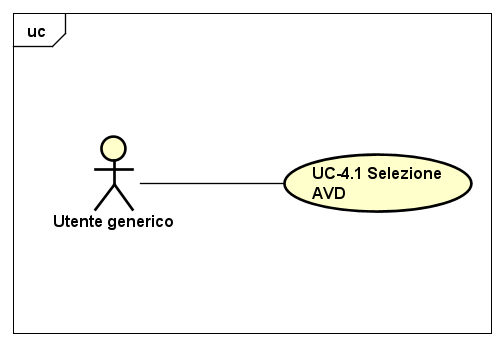
\includegraphics[width=10cm, height=8cm]{./usecase/uc_4_1.png}
    \caption{Sottocaso d'uso UC-4.1 Selezione AVD}
\end{figure}

\subsection*{UC-5 Visualizzazione messaggio nessun AVD rilevato} \label{subsec:uc-5-visualizzazione-messaggio-nessun-avd-rilevato}
\begin{itemize}
    \item \textbf{attori:} utente generico;
    \item \textbf{descrizione:} quando non sono presenti nessun AVD o il tool non è riuscito a rilevarne, viene mostrato un messaggio all'utente;
    \item \textbf{pre-condizioni:} l'utente ha aperto il tool;
    \item \textbf{post-condizioni:} l'utente ha visualizzato il messaggio;
    \item \textbf{flusso degli eventi principali:}
    \begin{itemize}
        \item l'utente visualizza il messaggio;
    \end{itemize}
\end{itemize}
\subsection*{UC-6 Errore durante avvio dell'AVD}\label{subsec:uc-6-errore-durante-avvio-dell'avd}
\begin{itemize}
    \item \textbf{attori:} utente generico;
    \item \textbf{descrizione:} serve a mostrare all'utente gli eventuali errori durante l'avvio dell'AVD;
    \item \textbf{pre-condizioni:} l'utente ha selezionato un'AVD e ha confermato l'avvio;
    \item \textbf{post-condizioni:} l'utente ha visualizzato il messaggio d'errore;
    \item \textbf{flusso degli eventi principali:}
    \begin{itemize}
        \item l'utente visualizza il messaggio d'errore;
    \end{itemize}
\end{itemize}
\subsection*{UC-7 Dump dello storage interno}\label{subsec:uc-6-dump-dello-storage-interno}
\begin{itemize}
    \item \textbf{attori:} utente generico;
    \item \textbf{descrizione:} nel caso l'utente volesse una copia dei dati interni dell'applicativo, ha bisogno di fare il dump;
    \item \textbf{pre-condizioni:} l'installazione dell'APK manomesso è andato a buon fine;
    \item \textbf{post-condizioni:} è stato fatto una copia dello storage interno;
    \item \textbf{flusso degli eventi principali:}
    \begin{itemize}
        \item l'utente seleziona la voce "copia i dati interni";
        \item l'utente seleziona il path dove collocare i dati;
    \end{itemize}
\end{itemize}
\subsection*{UC-8 Decodifica del codice}\label{subsec:uc-8-decodifica-del-codice}
\begin{itemize}
    \item \textbf{attori:} utente generico;
    \item \textbf{descrizione:} durante la decompilazione dell'APK vengono creati dei file .dex che contengono il codice sorgente dell'APK, e questo caso d'uso serve per permettere all'utente di ottenere il codice sorgente;
    \item \textbf{pre-condizioni:} la decompilazione è avvenuto con successo;
    \item \textbf{post-condizioni:} l'utente ha ottenuto una copia del codice sorgente in java;
    \item \textbf{flusso degli eventi principali:}
    \begin{itemize}
        \item l'utente ha selezionato la funzionalità decodifica dei dex;
        \item l'utente seleziona il percorso dove posizionare il codice sorgente ottenuto;
        \item l'utente ha salvato il codice sorgente ottenuto.
    \end{itemize}
\end{itemize}
\subsubsection*{UC-8.1 Avvio decodifica}
\begin{itemize}
    \item \textbf{attori:} utente generico;
    \item \textbf{descrizione:} serve all'utente per avviare la decodifica dei file .dex;
    \item \textbf{pre-condizioni:} la decompilazione dell'APK è avvenuto correttamente;
    \item \textbf{post-condizioni:} la decodifica è avvenuto con successo;
    \item \textbf{flusso degli eventi principali:}
    \begin{itemize}
        \item l'utente seleziona la funzionalità di decodifica dei file .dex;
    \end{itemize}
\end{itemize}
\subsubsection*{UC-8.2 Salvataggio del codice decodificato}
\begin{itemize}
    \item \textbf{attori:} utente generico;
    \item \textbf{descrizione:} serve all'utente per salvare i codici sorgenti decodificati;
    \item \textbf{pre-condizioni:} la decompilazione è avvenuto con successo;
    \item \textbf{post-condizioni:} i file con i codici sorgenti sono stati salvati correttamente;
    \item \textbf{flusso degli eventi principali:}
    \begin{itemize}
        \item l'utente seleziona la voce "salva file decodificati";
        \item l'utente seleziona la posizione dove vuole salvare i file;
        \item i file vengono salvati correttamente.
    \end{itemize}
\end{itemize}

\begin{figure}[H]
    \centering
    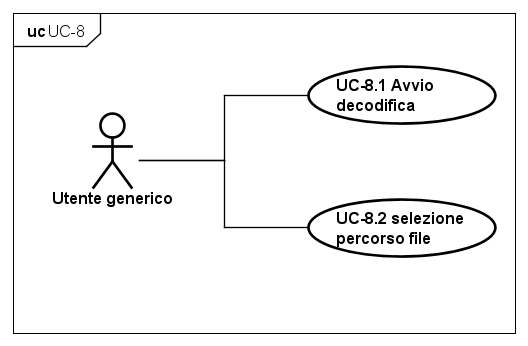
\includegraphics[width=10cm, height=8cm]{./immagini/usecase/uc_8.png}
    \caption{Caso d'uso UC-8 Decodifica codici .dex}
\end{figure}



\subsection*{UC-9 Visualizzazione errore decodifica}\label{subsec:uc-9-visualizzazione-errore-decodifica}
\begin{itemize}
    \item \textbf{attori:} utente generico;
    \item \textbf{descrizione:} durante la decodifica dei .dex possono sorgere molteplici errori;
    \item \textbf{pre-condizioni:} l'utente ha selezionato la funzionalità di decodifica del codice .dex;
    \item \textbf{post-condizioni:} l'utente ha visualizzato il messaggio di errore durante la decodifica;
    \item \textbf{flusso degli eventi principali:}
    \begin{itemize}
        \item l'utente ha visualizzato il messaggio d'errore;
    \end{itemize}
\end{itemize}

\begin{figure}[H]
    \centering
    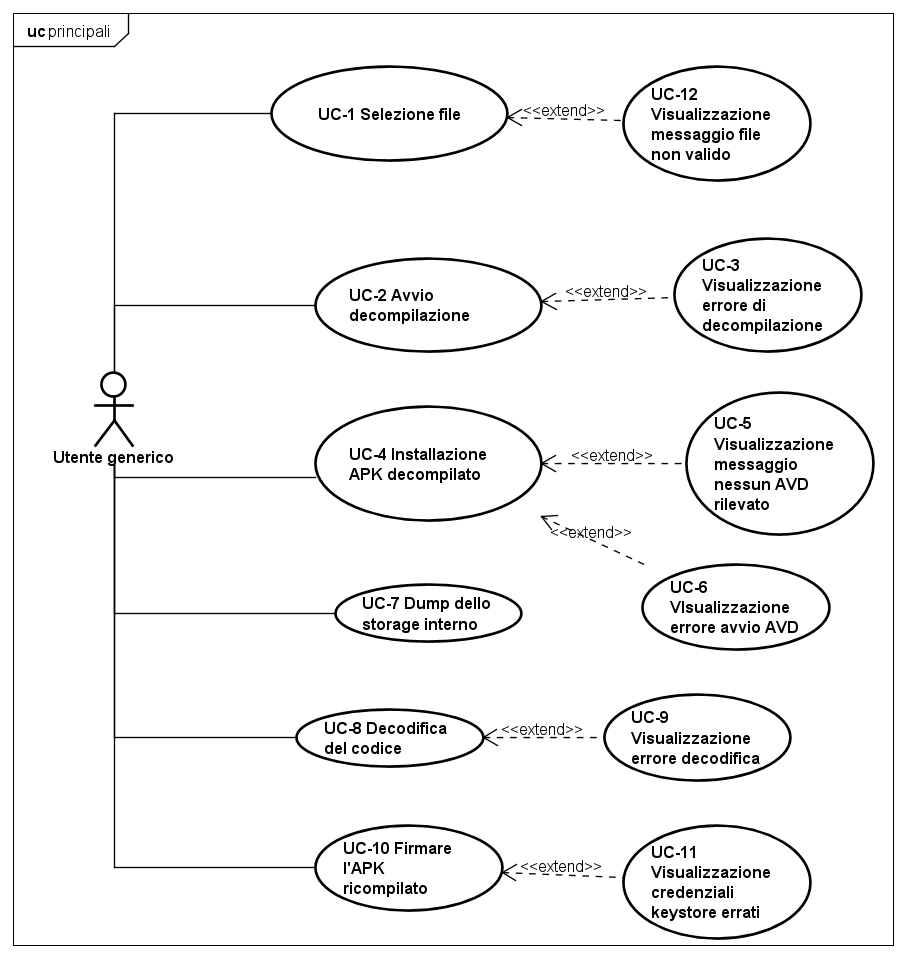
\includegraphics[width=10cm, height=8cm]{./immagini/usecase/uc_principali.png}
    \caption{Casi d'uso da 1 a 12}
\end{figure}

\subsection*{UC-10 Firmare l'APK ricompilato}\label{subsec:uc-10-firmare-l'apk-ricompilato}
\begin{itemize}
    \item \textbf{attori:} utente generico;
    \item \textbf{descrizione:} dopo la ricompilazione si può firmare l'APK;
    \item \textbf{pre-condizioni:} la ricompilazione dell'APK è avvenuto correttamente;
    \item \textbf{post-condizioni:} l'APK è stata firmata correttamente;
    \item \textbf{flusso degli eventi principali:}
    \begin{itemize}
        \item UC-10.1 selezione keystore;
        \item UC-10.3 inserimento alias;
        \item UC-10.4 inserimento password.
    \end{itemize}
    \item \textbf{Estensione}
    \begin{itemize}
        \item UC-11 Visualizzazione credenziali keystore errati;
    \end{itemize}
\end{itemize}
\subsubsection*{UC-10.1 Selezione keystore}\label{subsubsec:uc-10.1-selezione-keystore}
\begin{itemize}
    \item \textbf{attori:} utente generico;
    \item \textbf{descrizione:} permettere all'utente di selezionare il keystore da utilizzare per firmare l'APK;
    \item \textbf{pre-condizioni:} la ricompilazione dell'APK è avvenuto correttamente;
    \item \textbf{post-condizioni:} è stato selezionato un file di tipo keystore corretto (estensione: \textbf{.jks});
    \item \textbf{flusso degli eventi principali:}
    \begin{itemize}
        \item l'utente seleziona la funzionalità per selezionare il keystore;
        \item l'utente seleziona il keystore;
    \end{itemize}
    \item \textbf{flussi secondari}
    \begin{itemize}
        \item UC-10.2 Visualizzazione messaggio file selezionato non valido;
    \end{itemize}
\end{itemize}
\subsubsection*{UC-10.2 Visualizzazione messaggio file selezionato non valido}
\begin{itemize}
    \item \textbf{attori:} utente generico;
    \item \textbf{descrizione:} l'utente, al quale è stato chiesto di selezionare un file di tipo keystore, potrebbe selezionare un file non valido;
    \item \textbf{pre-condizioni:} l'utente ha selezionato un file;
    \item \textbf{post-condizioni:} il messaggio di errore è stato mostrato;
    \item \textbf{flusso degli eventi principali:}
    \begin{itemize}
        \item l'utente visualizza il messaggio d'errore.
    \end{itemize}
\end{itemize}
\subsubsection*{UC-10.3 Inserimento Alias}
\begin{itemize}
    \item \textbf{attori:} utente generico;
    \item \textbf{descrizione:} l'utente deve inserire l'alias della chiave da utilizzare durante la firma dell'APK;
    \item \textbf{pre-condizioni:} l'utente ha selezionato un keystore valido;
    \item \textbf{post-condizioni:} l'utente ha inserito l'alias da utilizzare;
    \item \textbf{flusso degli eventi principali:}
    \begin{itemize}
        \item l'utente inserisce l'alias della chiave da utilizzare per firmare l'APK;
    \end{itemize}
\end{itemize}
\subsubsection*{UC-10.4 Inserimento password}
\begin{itemize}
    \item \textbf{attori:} utente generico;
    \item \textbf{descrizione:} l'utente deve inserire la password del keystore da utilizzare durante la firma dell'APK;
    \item \textbf{pre-condizioni:} l'utente ha selezionato un keystore valido;
    \item \textbf{post-condizioni:} l'utente ha inserito la password da utilizzare;
    \item \textbf{flusso degli eventi principali:}
    \begin{itemize}
        \item l'utente inserisce la password;
    \end{itemize}
\end{itemize}
\begin{figure}[H]
    \centering
    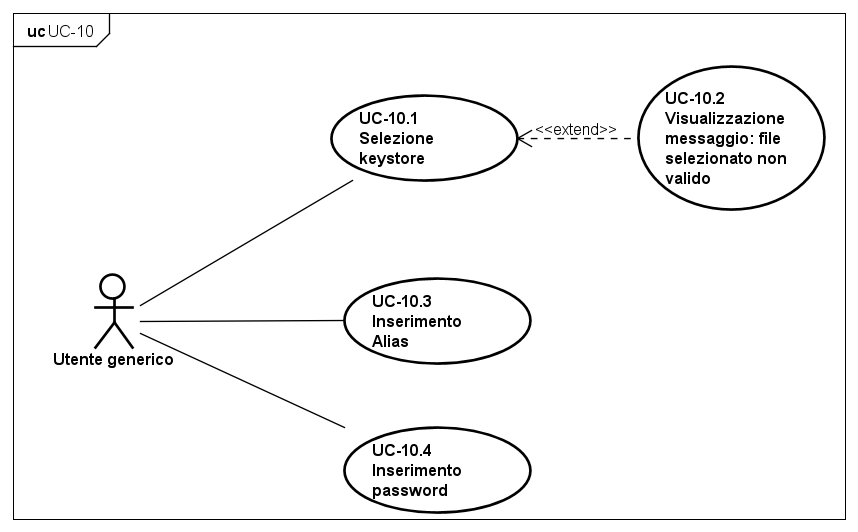
\includegraphics[width=10cm, height=8cm]{./immagini/usecase/uc_10.png}
    \caption{Sottocasi d'uso del caso d'uso UC-10}
\end{figure}

\subsection*{UC-11 Visualizzazione credenziali keystore errati}\label{subsec:uc-11-visualizzazione-credenziali-keystore-errati}
\begin{itemize}
    \item \textbf{attori:} utente generico;
    \item \textbf{descrizione:} per firmare l'APK l'utente deve inserire dei credenziali, e quando quest'ultimi sono errati viene mostrato un messaggio di errore;
    \item \textbf{pre-condizioni:} l'utente ha selezionato la funzionalità per ricompilare l'APK;
    \item \textbf{post-condizioni:} l'utente ha visualizzato il messaggio di errore;
    \item \textbf{flusso degli eventi principali:}
    \begin{itemize}
        \item l'utente ha visualizzato l'errore;
    \end{itemize}
\end{itemize}

\subsection*{UC-12 Visualizzazione messaggio file non valido}\label{subsec:uc-12-visualizzazione-messaggio-file-non-valido}
\begin{itemize}
    \item \textbf{attori:} utente generico;
    \item \textbf{descrizione:} quando l'utente seleziona un file che non ha l'estensione APK un messaggio deve essere mostrato all'utente;
    \item \textbf{pre-condizioni:} l'utente ha selezionato un file non APK;
    \item \textbf{post-condizioni:} l'utente ha visualizzato il messaggio d'errore;
    \item \textbf{flusso degli eventi principali:}
    \begin{itemize}
        \item l'utente visualizza il messaggio d'errore.
    \end{itemize}
\end{itemize}
\subsection*{UC-13 Decodifica dei file \textit{.dex} in file \textit{.java}}\label{subsec:uc-13-decodifica-dei-filetextitin-filetextit}
\begin{itemize}
    \item \textbf{attori:} utente generico;
    \item \textbf{descrizione:} dall'APK ricompilato si ottengono dei file \textit{.dex} che possono essere convertiti in \textit{.class} e quindi in \textit{.java};
    \item \textbf{pre-condizioni:} la decompilazione dell'APK \`{e} andata a buon fine;
    \item \textbf{post-condizioni:} la decodifica dei file \textit{.dex} in \textit{.java} \`{e} andata a buon fine;
    \item \textbf{flusso degli eventi principali:}
    \begin{itemize}
        \item l'utente seleziona la voce "Decodifica Dex".
    \end{itemize}
\end{itemize}

\subsection*{UC-14 Analisi del codice \textit{.java}}\label{subsec:uc-14-analisi-del-codicetextit}
\begin{itemize}
    \item \textbf{attori:} attore generico;
    \item \textbf{descrizione:} dopo aver ottenuto i file \textit{.java} eseguendo il caso d'uso UC-13, si potr\`{a} effettuare dell'analisi sul codice;
    \item \textbf{pre-condizioni:} la decodifica dei file \textit{.dex} in \textit{.java} \`{e} andata a buon fine;
    \item \textbf{post-condizioni:} viene generato un pdf con i risultati dell'analisi;
    \item \textbf{flusso degli eventi principali:}
    \begin{itemize}
        \item l'utente seleziona la voce "analyze";
        \item l'utente seleziona le opzioni di analisi;
        \item all'analisi completato, l'utente specifica dove posizionare il file pdf con i risultati dell'analisi;
        \item il file viene salvato nel percorso da lui specificato.
    \end{itemize}
\end{itemize}
\begin{figure}[H]
    \centering
    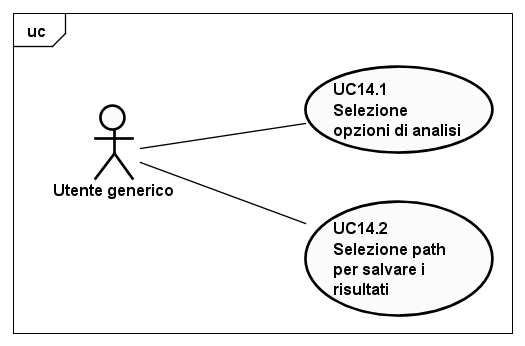
\includegraphics[width=10cm, height=8cm]{./immagini/usecase/uc_14_1_14_2.png}
    \caption{Sottocasi d'uso del caso d'uso 14}
\end{figure}



\subsection*{UC-15 avvio AVD}\label{subsec:uc-15-avvio-avd}
\begin{itemize}
    \item \textbf{attori:} attore generico;
    \item \textbf{descrizione:} serve per avviare un'avd per poter eseguire l'applicazione;
    \item \textbf{pre-condizioni:} il tool è stato avviato correttamente e nel sistema è presente almeno un AVD;
    \item \textbf{post-condizioni:} l'AVD è stato avviato correttamente;
    \item \textbf{flusso degli eventi principali:}
    \begin{itemize}
        \item l'attore visualizza l'elenco delle AVD presenti nel sistema;
        \item l'attore seleziona un'AVD che vuole avviare;
        \item l'attore seleziona se utilizzare un proxy da impostare nell'AVD;
        \item l'attore seleziona la voce avvia AVD.
    \end{itemize}
    \item \textbf{estensione:} UC-5 Visualizzazione messaggio nessun AVD rilevato.
\end{itemize}
\subsection*{UC-16 avvio AVD senza proxy}\label{subsec:uc-16-avvio-avd-senza-proxy}
\begin{itemize}
    \item \textbf{attori:} attore generico;
    \item \textbf{descrizione:} quando l'attore decide che non vuole avviare l'AVD modificando le impostazioni di proxy, viene eseguito questo caso d'uso;
    \item \textbf{pre-condizioni:} l'attore ha avviato correttamente il tool e nel sistema è presente almeno un'AVD;
    \item \textbf{post-condizioni:} l'AVD è stato avviato correttamente con le impostazioni di proxy di default;
    \item \textbf{flusso degli eventi principali:}
    \begin{itemize}
        \item l'attore visualizza l'elenco delle AVD presenti nel sistema;
        \item l'attore seleziona un'AVD che vuole avviare;
        \item l'attore seleziona di non utilizzare un proxy da impostare nell'AVD;
        \item l'attore seleziona la voce avvia AVD.
    \end{itemize}
\end{itemize}
\subsection*{UC-17 avvio AVD con proxy}\label{subsec:uc-16-avvio-avd-con-proxy}
\begin{itemize}
    \item \textbf{attori:} attore generico;
    \item \textbf{descrizione:} quando l'attore decide che non vuole avviare l'AVD modificando le impostazioni di proxy, viene eseguito questo caso d'uso;
    \item \textbf{pre-condizioni:} l'attore ha avviato correttamente il tool e nel sistema è presente almeno un'AVD;
    \item \textbf{post-condizioni:} l'AVD è stato avviato correttamente con le impostazioni di proxy inseriti;
    \item \textbf{flusso degli eventi principali:}
    \begin{itemize}
        \item l'attore visualizza l'elenco delle AVD presenti nel sistema;
        \item l'attore seleziona un'AVD che vuole avviare;
        \item l'attore seleziona di utilizzare un proxy da impostare nell'AVD;
        \item l'attore inserisce le informazioni del proxy, per esempio: \textit{localhost:8080};
        \item l'attore seleziona la voce avvia AVD.
    \end{itemize}
\end{itemize}
\subsubsection*{UC-17.1 Selezione voce Avvia con proxy}
\begin{itemize}
    \item \textbf{attori:} attore generico;
    \item \textbf{descrizione:} l'utente vuole avviare l'AVD con le opzioni di proxy;
    \item \textbf{pre-condizioni:} il tool è stato avviato correttamente ed è riuscito a rilevare gli AVD presenti nel sistema;
    \item \textbf{post-condizioni:} l'opzione di proxy è stato selezionato;
    \item \textbf{flusso degli eventi principali:}
    \begin{itemize}
        \item l'utente seleziona la voce per avviare l'AVD.
    \end{itemize}
\end{itemize}
\subsubsection*{UC-17.2 selezione voce avvio AVD}
\begin{itemize}
    \item \textbf{attori:} attore generico;
    \item \textbf{descrizione:} l'utente avviare l'AVD;
    \item \textbf{pre-condizioni:} l'utente ha selezionato le opzioni per avviare l'AVD;
    \item \textbf{post-condizioni:} il tool avvia l'AVD;
    \item \textbf{flusso degli eventi principali:}
    \begin{itemize}
        \item il tool seleziona la voce avvio di avviare l'AVD.
    \end{itemize}
\end{itemize}
\subsubsection*{UC-17.3 inserimento indirizzo e porta proxy}
\begin{itemize}
    \item \textbf{attori:} attore generico;
    \item \textbf{descrizione:} serve all'attore per inserire i dati del proxy;
    \item \textbf{pre-condizioni:} l'utente ha selezionato l'opzione di avviare l'AVD con il proxy;
    \item \textbf{post-condizioni:} i dati sono stati inseriti correttamente;
    \item \textbf{flusso degli eventi principali:}
    \begin{itemize}
        \item l'utente inserisce l'indirizzo IP del server proxy;
        \item l'utente inserisce il numero della porta del server proxy.
    \end{itemize}
\end{itemize}
\subsubsection*{UC-17.4 conferma dei dati}
\begin{itemize}
    \item \textbf{attori:} attore generico;
    \item \textbf{descrizione:} serve all'utente per confermare i dati inseriti per avviare l'AVD;
    \item \textbf{pre-condizioni:} l'utente ha inserito le opzioni di proxy correttamente;
    \item \textbf{post-condizioni:} l'AVD è stato avviato correttamente con le opzioni di proxy;
    \item \textbf{flusso degli eventi principali:}
    \begin{itemize}
        \item l'utente conferma le informazioni inserite e avvia l'AVD.
    \end{itemize}
\end{itemize}

\begin{figure}[H]
    \centering
    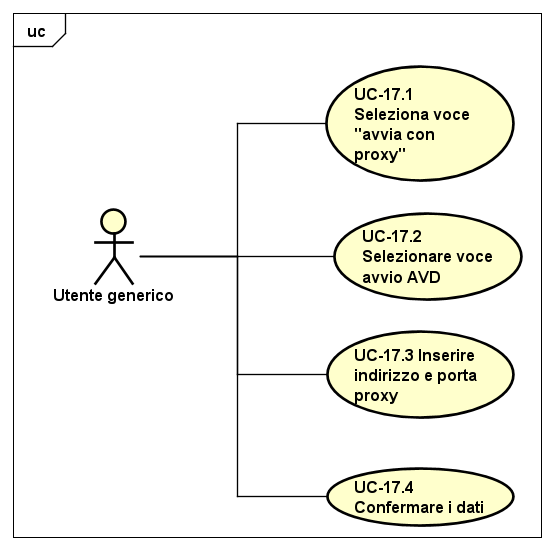
\includegraphics[width=10cm, height=8cm]{./immagini/usecase/uc_17.png}
    \caption{Sottocasi d'uso del caso d'uso 17}
\end{figure}
\subsection*{UC-18 Inizio registrazione traffico di rete}\label{subsec:uc-18-inizio-registrazione-traffico-di-rete}
\begin{itemize}
    \item \textbf{attori:} attore generico;
    \item \textbf{descrizione:} quando l'utente vuole registrare le attività di rete effettuate dall'AVD eseguendo l'applicazione, può utilizzare questa funzionalità;
    \item \textbf{pre-condizioni:} l'attore ha avviato l'applicazione;
    \item \textbf{post-condizioni:} l'attore ha registrato le attività di rete e ottenuto un file cap;
    \item \textbf{flusso degli eventi principali:}
    \begin{itemize}
        \item l'attore seleziona la voce "Start record!";
        \item l'attore successivamente seleziona la voce "Stop Record".
    \end{itemize}
\end{itemize}
\begin{figure}[H]
    \centering
    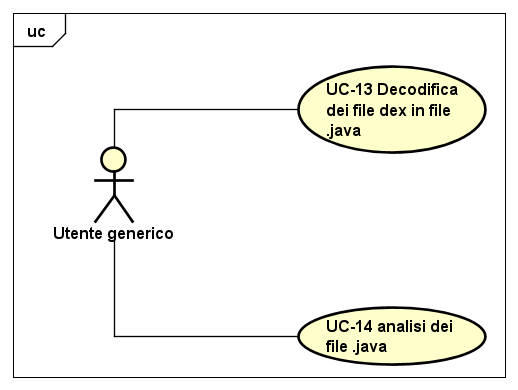
\includegraphics[width=10cm, height=8cm]{./immagini/usecase/UC-13_14.png}
    \caption{Casi d'uso da 13 a 18}
\end{figure}

%\subsection*{UC-}
%\begin{itemize}
%    \item \textbf{attori:} attore generico;
%    \item \textbf{descrizione:}
%    \item \textbf{pre-condizioni:}
%    \item \textbf{post-condizioni:}
%    \item \textbf{flusso degli eventi principali:}
%    \begin{itemize}
%    \end{itemize}
%\end{itemize}
\section{Tracciamento dei requisiti}\label{sec:tracciamento-dei-requisiti}
\newcounter{rowcount}
\setcounter{rowcount}{0}
\newcounter{subCount}
\setcounter{subCount}{0}

\subsection{Classificazione}\label{subsec:classificazione}
Di seguito sono riportati i requisiti individuati durante l'attività di analisi.
Tali requisiti sono stati individuati dai casi d'uso, dal piano di lavoro e dai colloqui con il tutor aziendale \tutorAziendale.
I requisiti individuati sono stati divisi in:
\begin{itemize}
    \item \textbf{Requisiti funzionali:} insieme di requisiti che definiscono le azioni fondamentali che devono avvenire in grado di processare un input e di generare un output;
    \item \textbf{Requisiti dichiarativi:} insieme di requisiti che rappresentano un vincolo di natura realizzativa, normativa o contrattuale;
    \item \textbf{Requisiti qualitativi:} insieme di requisiti che garantiscono una certa qualità al prodotto e che indicano le best practice usate per la realizzazione.
\end{itemize}
Inoltre, a ogni requisito è stata assegnata un'importanza:
\begin{itemize}
    \item \textbf{Obbligatori:} requisito al quale non si può rinunciare, indispensabile per il corretto funzionamento del prodotto;
    \item \textbf{Desiderabile:} requisito non necessario ma che porta valore aggiunto al prodotto;
    \item \textbf{Facoltativo:} requisito che risulta essere relativamente utile oppure contrattabile con il proponente in un momento successivo.
\end{itemize}

\subsection{Requisiti funzionali}\label{subsec:requisiti-funzionali}
Di seguiti sono elencati i requisiti derivanti dai casi d'uso individuati dalla sezione precedente.
\begin{longtable}{ | c| C{7cm} |C{3cm} |}
    \hline
    \textbf{Identificativo} & \textbf{Descrizione}                                                                                                  & \textbf{Fonte} \\\hline
    \idRequisiti{F-O}       & Il tool deve permettere di selezionare un file APK.                                                                   & UC-1           \\\hline
    \idRequisitiSub{F-O}    & Il tool deve permettere di mostrare un messaggio di errore se file selezionato non è valido.                          & UC-1           \\\hline
    \setcounter{subCount}{0}

    \idRequisiti{F-O}       & Il tool deve permettere di avviare la decompilazione dell'APK selezionato.                                            & UC-2           \\\hline
    \idRequisitiSub{F-O}    & Il tool deve permettere di visualizzare un messaggio di decompilazione avvenuto con successo.                         & UC-2           \\\hline
    \idRequisitiSub{F-O}    & Il tool deve aggiungere il flag android:debuggable="true" nel AndroidManifest.xml del decompilato.                    & UC-2           \\\hline
    \setcounter{subCount}{0}

    \idRequisiti{F-O}       & Il tool deve permettere di visualizzare il messaggio di errore quando la decompilazione non è terminato con successo. & UC-3           \\\hline
    \idRequisiti{F-O}       & Il tool deve permettere d'installare l'APK decompilato e modificato su un AVD.                                         & UC-4           \\\hline
    \idRequisitiSub{F-D}    & Il tool deve permettere di ricompilare l'APK decompilato.                                                             & UC-4           \\\hline
    \idRequisitiSub{F-D}    & Il tool deve permettere di avviare l'applicazione.                                                                    & UC-4           \\\hline
%        \setcounter{subCount}{0}

    \idRequisitiSub{F-O}    & Il tool deve permettere di selezionare un'AVD presente nel sistema.                                                   & UC-4           \\\hline
    \idRequisitiSub{F-O}    & Il tool deve permettere di visualizzare l'elenco delle AVD presenti nel sistema operativo.                            & UC-4           \\\hline
    \idRequisitiSub{F-O}    & Il tool deve permettere di confermare la selezione dell'AVD.                                                          & UC-4           \\\hline
    \setcounter{subCount}{0}

    \idRequisiti{F-O}       & Il tool deve permettere di visualizzare il messaggio quando non sono stati rilevati nessun AVD.                       & UC-5           \\\hline
    \idRequisiti{F-O}       & Il tool deve permettere di visualizzare il messaggio di errore se l'AVD selezionato non si è avviato correttamente.   & UC-6           \\\hline
    \idRequisiti{F-O}       & Il tool deve permettere di fare il dump dello storage interna dell'applicazione.                                      & UC-7           \\\hline
    \idRequisitiSub{F-O}    & Il tool deve permettere di selezionare il path dove collocare i dati copiati.                                         & UC-7           \\\hline
    \setcounter{subCount}{0}

    \idRequisiti{F-D}       & Il tool deve permettere di visualizzare i dex ottenuti dalla decompilazione.                                          & UC-8           \\\hline
    \idRequisitiSub{F-O}    & Il tool deve permettere di visualizzare il messaggio quando la decodifica è avvenuta con successo.                    & UC-8           \\\hline
    \idRequisitiSub{F-O}    & Il tool deve permettere di far selezionare il dex che l'utente vuole decodificare.                                    & UC-8           \\\hline
    \idRequisitiSub{F-O}    & Il tool deve permettere di confermare la selezione del dex da decodificare.                                           & UC-8           \\\hline
    \idRequisitiSub{F-O}    & Il tool deve permettere di far selezionare il path di dove salvare i file ottenuti dalla decodifica.                  & UC-8           \\\hline
    \setcounter{subCount}{0}

    \idRequisiti{F-O}       & Il tool deve permettere di visualizzare il messaggio d'errore se la decodifica non è andato a buon fine.              & UC-9           \\\hline

    \idRequisiti{F-F}       & Il tool deve permettere di firmare l'APK ricompilato.                                                                 & UC-10          \\\hline
    \idRequisitiSub{F-F}    & Il tool deve permettere di selezionare un file di tipo keystore.                                                      & UC-10          \\\hline
    \idRequisitiSub{F-F}    & Il tool deve permettere di mostrare un messaggio di errore quando viene selezionato un file non keystore.             & UC-10          \\\hline
    \idRequisitiSub{F-F}    & Il tool deve permettere d'inserire l'alias della chiave da utilizzare.                                                & UC-10          \\\hline
    \idRequisitiSub{F-F}    & Il tool deve permettere d'inserire la password del keystore da utilizzare.                                            & UC-10          \\\hline
    \setcounter{subCount}{0}

    \idRequisiti{F-F}       & Il tool deve permettere di mostrare dei messaggi quando le credenziali inseriti non sono corretti.                    & UC-11          \\\hline
    \idRequisiti{F-O}       & Il tool deve permettere di mostrare dei messaggi quando è stato selezionato un file non valido.                       & UC-12          \\\hline
    \idRequisiti{F-O}       & Il tool deve permettere di decodificare i file \textit{.dex} in \textit{.java}                                        & UC-13          \\\hline
    \idRequisiti{F-O}       & Il tool deve permettere di permettere di effettuare dell'analisi del codice java                                      & UC-14          \\\hline
    \idRequisitiSub{F-O}    & Il tool deve permettere di selezionare diverse opzioni di analisi                                                     & UC-14.1        \\\hline
    \idRequisitiSub{F-O}    & Il tool deve permettere di selezionare il path dove collocare i risultati dell'analisi.                               & UC-14.2        \\\hline
    \setcounter{subCount}{0}

    \idRequisiti{F-D}       & Il tool deve permettere di avviare un'AVD presente nel sistema.                                                       & UC-15          \\\hline
    \idRequisitiSub{F-D}    & Il tool deve permettere di visualizzare l'elenco delle AVD presenti nel sistema operativo.                            & UC-15          \\\hline
    \idRequisitiSub{F-D}    & Il tool deve permettere di selezionare un'AVD presente nel sistema.                                                   & UC-15          \\\hline
    \idRequisitiSub{F-D}    & Il tool deve permettere di specificare se avviare l'AVD con opzione di proxy.                                         & UC-15          \\\hline
    \setcounter{subCount}{0}
    \idRequisiti{F-D}       & Il tool deve permettere d'inserire le informazioni per il proxy.                                                      & UC-17          \\\hline
    \idRequisitiSub{F-D}    & Il tool deve permettere d'inserire l'indirizzo del server proxy.                                                      & UC-17          \\\hline
    \idRequisitiSub{F-D}    & Il tool deve permettere d'inserire il numero di porta del server proxy.                                               & UC-17          \\\hline
    \setcounter{subCount}{0}
    \idRequisiti{F-D}       & Il tool deve permettere di registrare il traffico di rete.                                                            & UC-18          \\\hline
    \idRequisitiSub{F-D}    & Il tool deve generare il file che contiene i dettagli del traffico di rete.                                           & UC-18          \\\hline
    \caption{Requisiti funzionali}
\end{longtable}

\setcounter{rowcount}{0}

\subsection{Requisiti di vincolo}\label{subsec:requisiti-vincolo}
\begin{center}
    \begin{longtable}{ | c| C{7cm} |C{3cm} |}
        \hline
        \textbf{Identificativo} & \textbf{Descrizione}                                              & \textbf{Fonte}   \\\hline
        \idRequisiti{V-D}       & Il tool può essere un tool da righe di comando                   & Piano di lavoro. \\\hline
        \idRequisiti{V-D}       & Il tool può essere un tool dotato di GUI                          & Piano di lavoro. \\\hline
        \idRequisiti{V-D}       & Il tool può essere sviluppato in JAVA                             & Piano di lavoro. \\\hline
        \idRequisiti{V-F}       & Il tool può essere sviluppato utilizzando i linguaggi funzionali. & Piano di lavoro. \\\hline
        \caption{Requisiti di vincolo}
    \end{longtable}
\end{center}
\setcounter{rowcount}{0}

\subsection{Requisiti qualitativi}\label{subsec:requisiti-qualitativi}
\begin{center}
    \begin{longtable}{ | c| C{7cm} |C{3cm} |}
        \hline
        \textbf{Identificativo} & \textbf{Descrizione}                                                                           & \textbf{Fonte}  \\\hline
        \idRequisiti{Q-O}       & Il codice sorgente deve essere versionato col sistema di versionamento dell'azienda ospitante. & Piano di lavoro \\\hline
        \idRequisiti{Q-O}       & Il Il codice sorgente deve essere sotto licenza GPL v3.                                        & Piano di lavoro \\\hline
%        \idRequisiti{Q-O}&Il code coverage dei test unitari deve superare 80\%.& Piano di lavoro\\\hline
%        \idRequisiti{Q-D}&Il code coverage dei test unitari deve essere 100\%.& Piano di lavoro\\\hline
        \caption{Requisiti qualitativi}
    \end{longtable}
\end{center}
\setcounter{subCount}{0}
\setcounter{rowcount}{0}
\section{Tracciamento fonte - requisiti}\label{sec:tracciamento-fonte---requisiti}

\begin{center}
    \begin{longtable}{| C{6cm} |C{6cm}|}
        \hline
        \textbf{Fonte} & \textbf{Requisito} \\\hline
        UC-1 &
        \begin{itemize}\itemsep0em
            \item R-1-F-O
            \item R-1.1-F-O
        \end{itemize}
        \\\hline
        UC-2 &
        \begin{itemize}\itemsep0em
            \item R-2-F-O
            \item R-2.1-F-O
            \item R-2.2-F-O
        \end{itemize}
        \\\hline
        UC-3 &
        \begin{itemize}\itemsep0em
            \item R-3-F-O
        \end{itemize} \\\hline
        UC-4 &
        \begin{itemize}\itemsep0em
            \item R-4-F-O
            \item R-4.1-F-D
            \item R-4.2-F-D
            \item R-4.3-F-O
            \item R-4.4-F-O
            \item R-4.5-F-O
            \item R-4.6-F-O
        \end{itemize} \\\hline
        UC-5 &
        \begin{itemize}\itemsep0em
            \item R-6-F-O
        \end{itemize} \\\hline
        UC-6 &
        \begin{itemize}\itemsep0em
            \item R-7-F-O
        \end{itemize} \\\hline
        UC-7 &
        \begin{itemize}\itemsep0em
            \item R-8-F-O
            \item R-8.1-F-O
        \end{itemize} \\\hline
        UC-8 &
        \begin{itemize}\itemsep0em
            \item R-9-F-D
            \item R-9.1-F-O
            \item R-9.2-F-O
            \item R-9.3-F-O
        \end{itemize} \\\hline
        UC-8.2 &
        \begin{itemize}\itemsep0em
            \item R-9.4-F-O
        \end{itemize} \\\hline
        UC-9 & \begin{itemize}\itemsep0em
                   \item R-10-F-O
        \end{itemize} \\\hline
        UC-10 &
        \begin{itemize}\itemsep0em
            \item R-11-F-F
            \item R-11.1-F-F
            \item R-11.2-F-F
            \item R-11.3-F-F
            \item R-11.4-F-F
            \item R-11.4-F-F
        \end{itemize}
        \\\hline

        UC-11 &
        \begin{itemize}\itemsep0em
            \item R-12-F-F
        \end{itemize}
        \\\hline

        UC-12 &
        \begin{itemize}\itemsep0em
            \item R-13-F-O
        \end{itemize}
        \\\hline

        UC-13 &
        \begin{itemize}\itemsep0em
            \item R-14-F-O
        \end{itemize} \\\hline
        UC-14 &
        \begin{itemize}\itemsep0em
            \item R-15-F-O
            \item R-15.1-F-O
            \item R-15.2-F-O
        \end{itemize} \\\hline

        UC-15 &
        \begin{itemize}\itemsep0em
            \item R-16-F-D
            \item R-16.1-F-D
            \item R-16.2-F-D
            \item R-16.3-F-D
        \end{itemize} \\\hline
        UC-17 &
        \begin{itemize}\itemsep0em
            \item R-17-F-D
            \item R-17.1-F-D
            \item R-17.2-F-D
        \end{itemize} \\\hline
        UC-18 &
        \begin{itemize}\itemsep0em
            \item R-18-F-D
            \item R-18.1-F-D
            \item R-18.2-F-D
            \item R-18.3-F-D
        \end{itemize} \\\hline
        Colloquio col tutor azienda &
        \begin{itemize}\itemsep0em
            \item R-1-V-D,
            \item R-2-V-D,
            \item R-3-V-D,
            \item R-4-V-F,
            \item R-1-Q-O,
            \item R-2-Q-O,
            \item R-3-Q-D,
            \item R-4-Q-O
        \end{itemize} \\\hline
        \caption{Tracciamento fonte - requisiti}
    \end{longtable}
\end{center}

\subsection{Tracciamento requisito - fonte}\label{subsec:tracciamento-requisiti---fonte}

\begin{longtable}{| C{6cm} |C{6cm}|}
    \hline
    \textbf{Requisito} & \textbf{Fonte}  \\\hline
    R-1-F-O            & UC-1            \\\hline
    R-1.1-F-O          & UC-1            \\\hline
    R-2-F-O            & UC-2            \\\hline
    R-2.1-F-O          & UC-2            \\\hline
    R-2.2-F-O          & UC-2            \\\hline
    R-3-F-O            & UC-3            \\\hline
    R-4-F-O            & UC-4            \\\hline
    R-4.1-F-D          & UC-4            \\\hline
    R-5-F-O            & UC-4.1          \\\hline
    R-5.1-F-O          & UC-4.1          \\\hline
    R-5.2-F-O          & UC-4.1          \\\hline
    R-5.3-F-O          & UC-4.1          \\\hline
    R-6-F-O            & UC-5            \\\hline
    R-7-F-O            & UC-6            \\\hline
    R-8-F-O            & UC-7            \\\hline
    R-8.1-F-O          & UC-7            \\\hline
    R-9-F-D            & UC-8            \\\hline
    R-9.1-F-O          & UC-8            \\\hline
    R-9.2-F-O          & UC-8.1          \\\hline
    R-9.3-F-O          & UC-8.1          \\\hline
    R-9.4-F-O          & UC-8.2          \\\hline
    R-10-F-O           & UC-9            \\\hline
    R-11-F-F           & UC-10           \\\hline
    R-11.1-F-F         & UC-10.1         \\\hline
    R-11.2-F-F         & UC-10.2         \\\hline
    R-11.3-F-F         & UC-10.3         \\\hline
    R-11.4-F-F         & UC-10.4         \\\hline
    R-12-F-F           & UC-11           \\\hline
    R-13-F-O           & UC-12           \\\hline
    R-14-F-O           & UC-13           \\\hline
    R-15-F-O           & UC-14           \\\hline
    R-15.1-F-O         & UC-14           \\\hline
    R-15.2-F-O         & UC-14           \\\hline
    R-16-F-D           & UC-15           \\\hline
    R-16.1-F-D         & UC-15           \\\hline
    R-16.2-F-D         & UC-15           \\\hline
    R-16.3-F-D         & UC-15           \\\hline
    R-17-F-D           & UC-17           \\\hline
    R-17.1-F-D         & UC-17           \\\hline
    R-17.2-F-D         & UC-17           \\\hline
    R-18-F-D           & UC-18           \\\hline
    R-18.1-F-D         & UC-18           \\\hline
    R-18.2-F-D         & UC-18           \\\hline
    R-18.3-F-D         & UC-18           \\\hline
    R-19-V-D            & Piano di lavoro \\\hline
    R-20-V-D            & Piano di lavoro \\\hline
    R-21-V-D            & Piano di lavoro \\\hline
    R-22-V-F            & Piano di lavoro \\\hline
    R-23-Q-O            & Piano di lavoro \\\hline
    R-24-Q-O            & Piano di lavoro \\\hline
%        R-2-Q-O& Piano di lavoro\\\hline
%        R-3-Q-D& Piano di lavoro\\\hline
    \caption{Tracciamento requisiti - fonte}
\end{longtable}




             % Concept Preview
    % !TEX encoding = UTF-8
% !TEX TS-program = pdflatex
% !TEX root = ../tesi.tex

%**************************************************************


\chapter{Progettazione e codifica}
\label{ch:progettazione-e-codifica}
%**************************************************************

\intro{In questo capitolo vengono presentate le tecnologie e gli strumenti utilizzati, il ciclo di sviluppo del software adottato e i design pattern utilizzati.}\\

% !TEX encoding = UTF-8
% !TEX TS-program = pdflatex
% !TEX root = ../tesi.tex

\section{Tecnologie}\label{sec:tecnologie}
Di seguito viene data una panoramica delle tecnologie e degli strumenti utilizzati.

\subsection*{CFR - decompilatore java}
CFR è il decompilatore utilizzato per trasformare il codice bytecode \textit{.class} in codice sorgente \textit{.java};
\url{http://www.benf.org/other/cfr/index.html}

\subsection*{Apk Tool}
Apktool è un tool per effettuare il reverse engineering delle applicazioni Android. Può decodificare le risorse contenute nell'APK in una forma quasi uguale a quelli originali, può anche di ricostruire l'APK dopo le modifiche alle risorse modificate.
\url{https://ibotpeaches.github.io/Apktool/}
\subsection*{Dex2Jar}
Questo strumento permette di trasformare i file \textit{.dex} in formato \textit{.jar} in modo che possa essere letta attraverso un software di compressione, come 7Zip, per poter accedere quindi ai file di tipo \textit{.class}.
\url{https://github.com/pxb1988/dex2jar}


\subsection*{Java}
In informatica, Java è un linguaggio di programmazione ad alto livello, orientato agli oggetti e tipizzazione statica, che si appoggia sull'omonima piattaforma software di esecuzione, specificamente progettato per essere il più possibile indipendente dalla piattaforma hardware di esecuzione.
\subsection*{Json}
JSON (JavaScript Object Notation) è un semplice formato per lo scambio di dati.
Per le persone è facile da leggere e scrivere, mentre per le macchine risulta facile da generare e analizzarne la sintassi.
JSON è basato su due strutture:
\begin{itemize}
    \item un insieme di coppie nome/valore, in diversi linguaggi, questo è realizzato come un oggetto, un record, uno struct, un dizionario, una tabella hash, un elenco di chiavi o un array associativo.
    \item un elenco ordinato di valori, nella maggior parte dei linguaggi questo si realizza con un array, un vettore o una sequenza.
\end{itemize}
\url{https://www.json.org/json-it.html}

\subsection*{XPath}\label{subsec:xpath}
In informatica XPath è un linguaggio, parte della famiglia XML, che permette di individuare i nodi all'interno di un documento XML. Le espressioni XPath, a differenza delle espressioni XML, non servono a identificare la struttura di un documento, bensì a localizzarne con precisione i nodi.


\section{Strumenti}\label{sec:strumenti}

\subsection*{Intellij IDEA}
L'IDE utilizzato per la scrittura del codice in Java sviluppato da JetBrains.
\url{https://www.jetbrains.com/idea/}

\subsection*{Android Emulator}
Lo strumento che permette di avviare degli emulatori Android, conosciuti anche come AVD. È stato utilizzato per eseguire l'applicazione ricompilata, per poter fare il dump dei dati presenti nell'area di storage dell'applicazione, come i file JSON, XML e SQLite, o come il file delle attività di rete.
\url{https://developer.android.com/studio/run/emulator}

\subsection*{Maven}
Maven è un tool di build automation, basato sul concetto di Project Object Model (POM), maven può gestire i build, fare il report e la documentazione da un singolo centro di informazione.
\url{https://maven.apache.org/}

\subsection*{Astah}
Astah è uno strumento di modellazione UML. Permette di creare vari diagrammi UML, come quelli di classe, di package, di sequenza e di attività.
\url{https://astah.net/products/astah-community/}

\subsection*{Git - GitLab}
Gitlab è una piattaforma web open-source che permette la gestione di repository e di funzioni d'issue tracking system.
Questa è un'istanza privata dell'azienda Imola Informatica S.p.A.
\url{https://git.imolinfo.it/users/sign_in}
% !TEX encoding = UTF-8
% !TEX TS-program = pdflatex
% !TEX root = ../tesi.tex

\section{Ciclo di vita del software}\label{sec:ciclo-vita-software}
Il modello adottato per lo sviluppo del progetto è il modello incrementale, permettendo così di suddividere la durata del progetto in diversi incrementi, in ognuno dei quali sono stati definiti degli obiettivi/requisiti da raggiungere.
Inoltre, tale modello di sviluppo ha come conseguenza i seguenti vantaggi:
\begin{itemize}
    \item assegnare diverse priorità agli obiettivi da raggiungere, in modo che quelli più importanti vengano raggiunti prima;
    \item è possibile mostrare il prodotto al termine di ogni incremento in questo modo si assicura che il risultato di ogni incremento sia consono alle aspettative del cliente;
    \item la fase di verifica avviene ad ogni incremento in modo da garantire la correttezza del prodotto di ogni incremento;
    \item a ogni incremento vengono aggiunte delle funzionalità corrette e funzionanti, allora il prodotto finale soddisfa i requisiti del cliente;
\end{itemize}
% !TEX encoding = UTF-8
% !TEX TS-program = pdflatex
% !TEX root = ../tesi.tex

\newpage %fixme
\section{Progettazione}
\label{sec:progettazione}

\subsection{Package}\label{subsec:package}
Questo è il root package del tool, contiene altri package e le due classi elencati successivamente.
\begin{namespacedesc}
    \classdesc{ApatLauncher}{È la classe di launcher del tool, si occupa principalmente di mettere in relazione di observed-observer i componenti della vista con i dati del modello;}
    \classdesc{Utils}{La classe di utilities che ha delle funzioni statiche utilizzata nel tool per evitare la ripetizione del codice.}
\end{namespacedesc}

\subsubsection{Package it.imolinfo.apat.controller} %**************************
Questo è il package che contiene la classe Controller e ciò che riguarda l'interazione del controller con il filesystem.
\begin{namespacedesc}
    \classdesc{AndroidManifestEditor.java}{È la classe che si occupa, dato un oggetto di tipo File Android Manifest, di modificare e/o aggiungere il tag \textit{debugabble} impostando il suo valore a \textit{true};}
    \classdesc{Controller}{È il controller del MVC, si occupa di effettuare le operazioni di decompilazione, ricompilazione, decodifica e analisi dei file;}
    \classdesc{MVCModule}{È la classe di effettuare la dependency injection per la creazione del MVC.}
\end{namespacedesc}

\subsubsection{Package it.imolinfo.apat.model} %**************************
Questo package contiene le classi che riguardano il modello del pattern Model View Controller.
\begin{namespacedesc}
    \classdesc{Modello}{La classe che contiene i dati utili al corretto funzionamento del tool;}
    \classdesc{ModelState}{È la classe che viene usato per poter salvare lo stato del funzionamento del tool. Lo stato viene salvato quando viene chiuso il tool, e viene ricaricato al successivo avvio;}
    \classdesc{PDFWriter}{È la classe wrapper che si occupa della creazione del file PDF per salvare i risultati dell'analisi;}
    \classdesc{Result}{È la classe di messaggio che viene restituita quando il tool interagisce con il file system;}
    \classdesc{Unzipper}{È la classe si occupa di decomprimere i file zip;}
    \classdesc{Dumper}{È la classe che si occupa di effettuare il dump dei dati da un file con estensione \textit{db};}
\end{namespacedesc}

\subsubsection{Package it.imolinfo.apat.pattern} %**************************
Questo package contiene degli sotto-package ognuno dei quali rappresenta un design pattern utilizzato nello sviluppo del tool.
I pattern utilizzati sono
\begin{namespacedesc}
    \classdesc{analyzer.Analyze}{È l'interfaccia di base del pattern Decorator.}
    \classdesc{analyzer.BaseAnalyzer}{È la classe dell'oggetto base che viene decorato.}
    \classdesc{analyzer.BaseAnalyzeDecorator}{È il classe astratta del decorator di base che implementa l'interfaccia Analyze, e ha un metodo astratto \textit{doAnalysis()} che deve essere implementato dai decorator concreti.}
    \classdesc{analyzer.DumpDataBase}{È il decorator che si occupa di estrarre i contenuti dei file \textit{.db} scaricati dall'area di storage dell'app.}
    \classdesc{analyzer.DumpedFilesAnalyzer}{È il decorator che si occupa di analizzare i file dell'area di storage dell'applicazione con estensione \textit{XML} e \textit{json}, principalmente, legge il contenuto di tali file, e in base ad una whitelist, seleziona quali risultati restituire al chiamante.}
    \classdesc{analyzer.LambdaCounter}{È il decorator che conta il numero di lambda presente per ogni classe di codice \textit{.java} decompilato.}
    \classdesc{analyzer.StringFinder}{È il decorator che analizza i file di tipo \textit{.java}, ed estrae le stringhe hardcoded, può essere utilizzato insieme a un blacklist delle stringhe che devono essere ignorate.}
\end{namespacedesc}
\begin{namespacedesc}
    \classdesc{observer.Observable}{La classe parametrizzata T che può essere osservato;}
    \classdesc{observer.Observer}{L'interfaccia parametrizzata che ha il ruolo dell'observer;}
\end{namespacedesc}
\begin{namespacedesc}
    \classdesc{CliCommandFactory.Commands}{È l'interfaccia che contiene i metodi, dove ognuno dei quali deve generare delle istruzioni per la linea di comando.}
    \classdesc{CliCommandFactory.CommandFactory}{È la classe astratta che implementa la precendente interfaccia, con un costruttore di base che richiede un path di base.}
    \classdesc{CliCommandFactory.UnixCommandFactory}{È l'implementazione della classe astratta CommandFactory per il sistema UNIX.}
    \classdesc{CliCommandFactory.WindowsCommandFactory}{È l'implementazione della classe astratta CommandFactory per il sistema Windows.}
\end{namespacedesc}

\subsubsection{Package it.imolinfo.apat.view} %**************************
\begin{namespacedesc}
    \classdesc{AnalysisChooser}{È la finestra che mostra le opzioni di analisi.}
    \classdesc{View}{È la finestra principale, dove permette di selezionare il file \textit{apk} da decompilare ed analizzare.}
    \classdesc{WaitAction}{È una classe astratta che a sua volta eredita dalla classe Action e permette di eseguire un processo mostrando la barra del caricamento.}
    \classdesc{ApkFilter}{È l'implementazione dell'interfaccia \textbf{FileFilter} che accetta solo i file di tipo \textit{APK}.}
    \classdesc{KeyStoreFilter}{È l'implementazione dell'interfaccia \textbf{FileFilter} che accetta solo i file di tipo \textit{JKS}.}
    \classdesc{TextFilter}{È l'implementazione dell'interfaccia \textbf{FileFilter} che accetta solo i file di tipo \textit{txt}.}
\end{namespacedesc}
% !TEX encoding = UTF-8
% !TEX TS-program = pdflatex
% !TEX root = ../tesi.tex
\section{Design Pattern utilizzati}\label{sec:design-pattern-utilizzati}
Di seguito, sono elencati i design pattern utilizzati durante la creazione del tool. Per ognuno di questi, verrà fornito il diagramma delle classi e una descrizione.
\subsection{Model View Controller}\label{subsec:model-view-controller}
Come pattern architetturale è stato adottato il pattern Model-View-Controller, poiché è in grado di separare la logica di presentazione dei dati dalla logica di business.\\
L'applicazione di tale pattern avviene attraverso il pattern Observer, nello specifico, le singole componenti della vista osservano i valori della classe Modello, in questo modo, quando il valore di un determinato attributo viene modificato, il nuovo valore viene notificato alla componente della vista.
\begin{figure}[H]
    \centering
    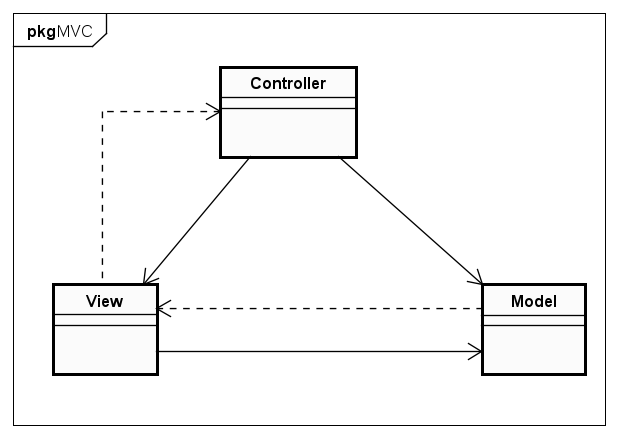
\includegraphics[width=13cm, height=8cm]{./immagini/diagrammi_uml/mvc.png}
    \caption{Diagramma delle classi del pattern MVC}\label{fig:mvc}
\end{figure}

\newpage
\subsection{Observer}\label{subsec:observer}
Il pattern observer permette di definire una dipendenza uno a molti fra oggetti, in modo tale che se un oggetto cambia il suo stato, tutti gli oggetti dipendenti da questo siano notificati e aggiornati automaticamente.\\
L'implementazione di tale pattern avviene attraverso una classe \textit{Observable} e un'interfaccia \textit{Observer} entrambe template, per modificare il valore dell'observable è sufficiente utilizzare il metodo \textit{setValue(newValue:T)}, in questo modo, su ogni elemento della lista \textit{observables} viene invocato il metodo \textit{onChanged} passando il nuovo valore.\\
Tale pattern viene applicato nel tool perché i componenti delle viste possano osservare il contenuto del modello.
\begin{figure}[H]
    \centering
    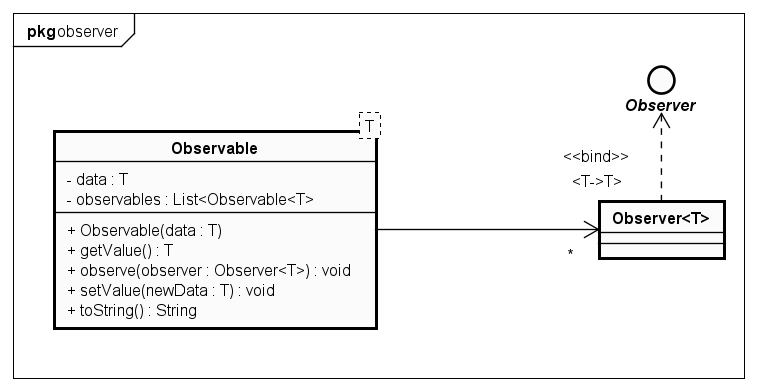
\includegraphics[width=13cm, height=8cm]{./immagini/diagrammi_uml/Observer.png}
    \caption{Diagramma delle classi del pattern Observer}\label{fig:observer}
\end{figure}

\newpage
\subsection{Decorator}\label{subsec:decorator}
Il pattern decorator è stato utilizzato per creare la parte del tool che si occupa di effettuare l'analisi del codice decompilato e dei file scaricati dall'area di storage dell'applicazione presenti nell'Android Emulator Device.\\
Il vantaggio ottenuto per aver utilizzato questo pattern è quello di poter "decorare" l'oggetto base di analisi, ovvero l'istanza della classe \textit{BaseAnalyzer} con i vari decorator, un altro importante vantaggio è quello di poter aggiungere altre funzionalità di analisi facilmente nel tool, infatti, è sufficiente creare un'altra sottoclasse della classe \textit{BaseAnalyzeDecorator} quindi implementare il metodo astratto.
\begin{figure}[H]
    \centering
    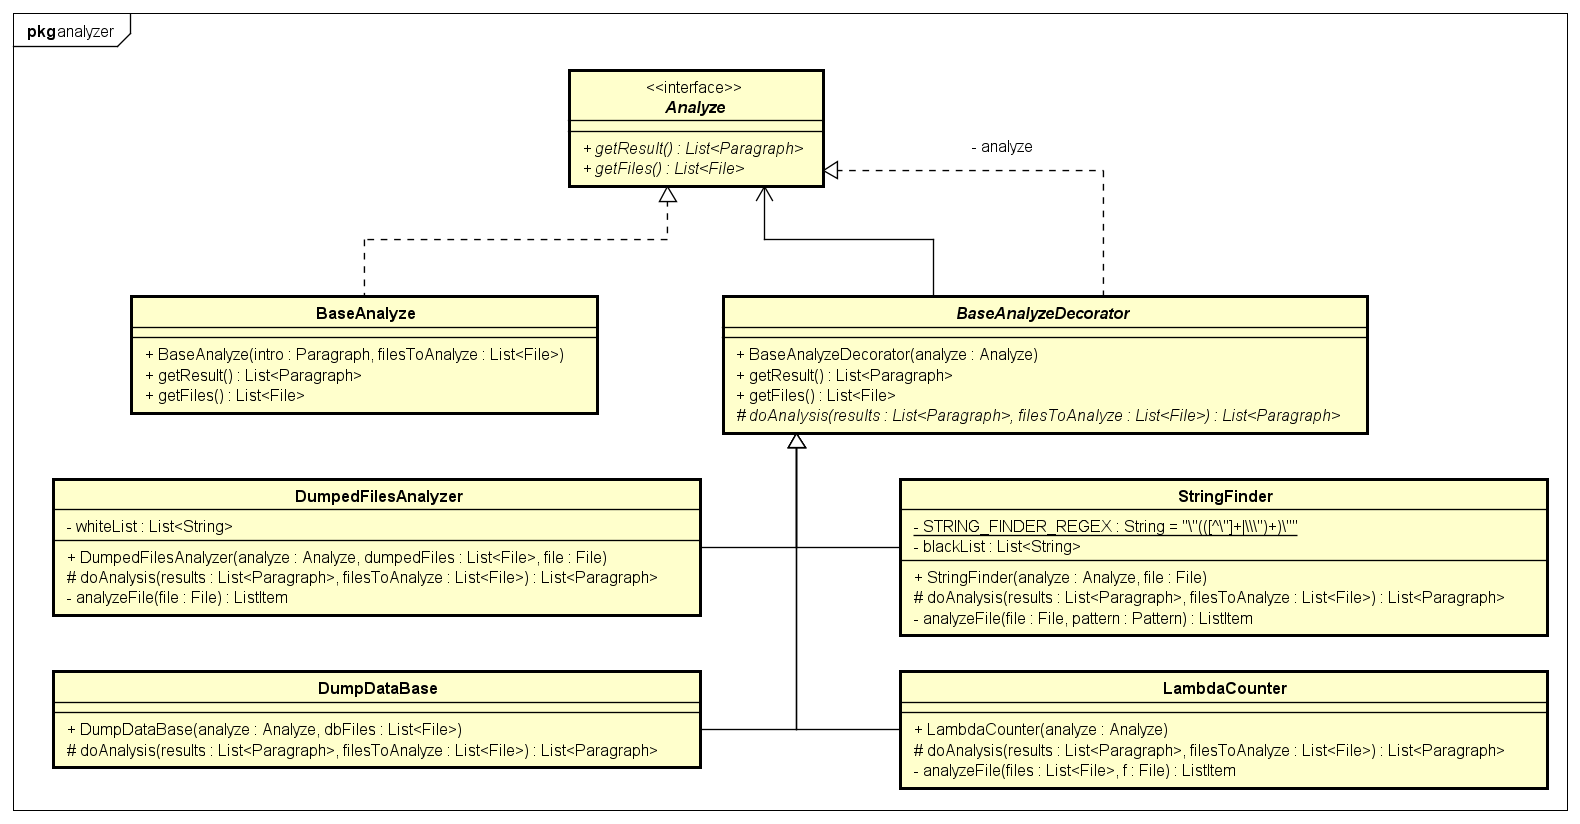
\includegraphics[width=13cm, height=10cm]{./immagini/diagrammi_uml/Decorator.png}
    \caption{Diagramma delle classi del pattern Decorator}\label{fig:decorator}
\end{figure}

\newpage
\subsection{Factory Method}\label{subsec:factory-method}
Questo pattern è stato utilizzato per poter fornire al controller dei comandi da eseguire nei processi, essendo i comandi dipendente dal sistema operativo, sono state create due classi, una per Windows chiamata \textit{WindowsCommandFactory} e una per Linux chiamata \textit{LinuxCommandFactory}.
Allo start-up del tool, viene letta una dalla JVM una variabile chiamata \textit{os.name}, e dipendentemente da valore letto, viene deciso quale delle sottoclassi istanziare per il corretto funzionamento del tool.
\begin{figure}[H]
    \centering
    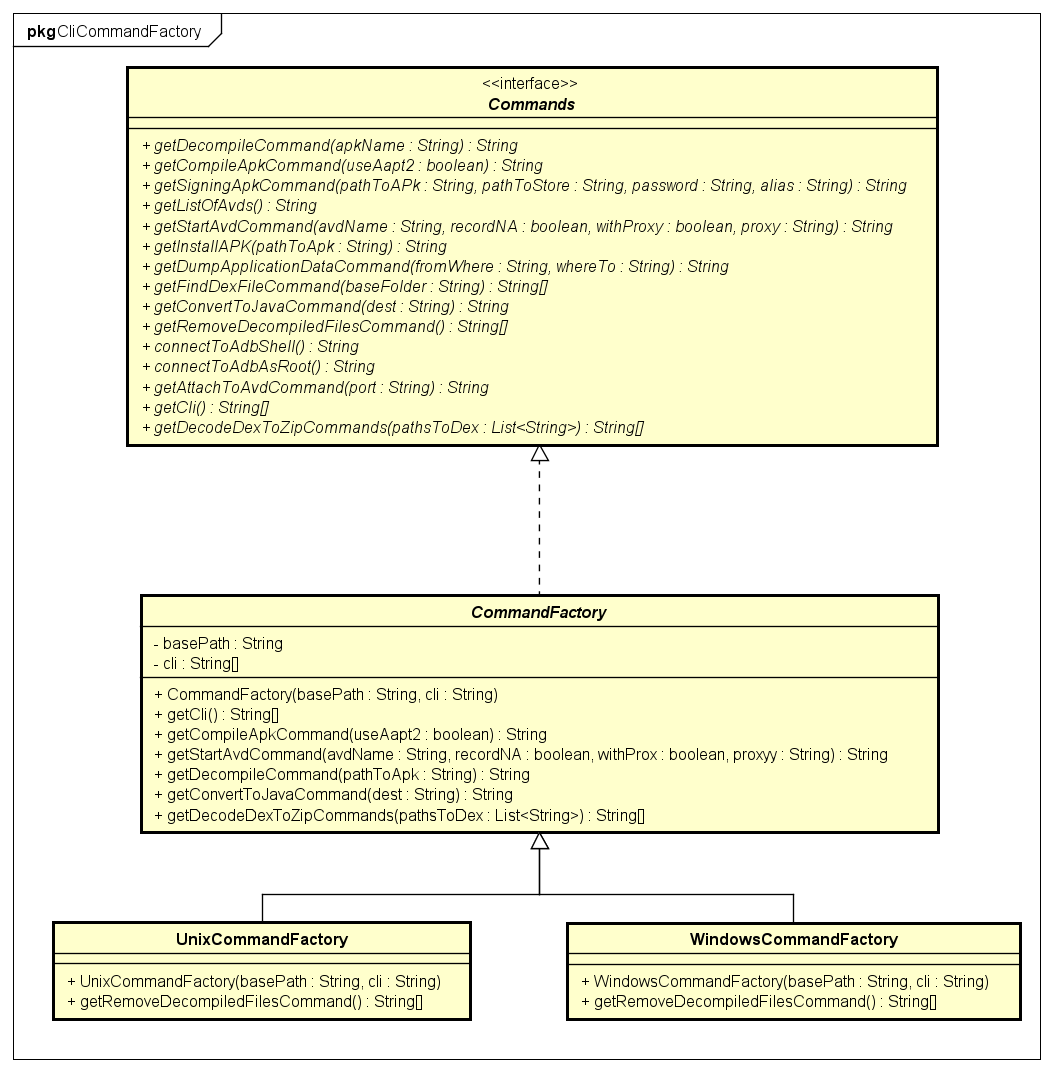
\includegraphics[width=14cm, height=14cm]{./immagini/diagrammi_uml/CommandFactory.png}
    \caption{Diagramma delle classi del pattern FactoryMethod}\label{fig:factory-method}
\end{figure}
% !TEX encoding = UTF-8
% !TEX TS-program = pdflatex
% !TEX root = ../tesi.tex

\section{Codifica}\label{sec:codifica}
Per la fase di codifica sono state adottate le seguenti convenzioni:
\begin{itemize}
    \item il nome delle classi seguirà la notazione a Cammello, un esempio corretto è: \textit{WindowsCommandFactory};
    \item il nome degli attributi seguirà sempre la notazione a Cammello, ma con la prima lettera in minuscolo, un esempio corretto è: \textit{commandsFactory};
    \item ove possibile, si deve utilizzare le espressioni lambda;
    \item la gestione delle eccezioni deve essere venir fatta sempre dal chiamante;
    \item per ogni classe e ogni metodo deve essere fornita una descrizione in JavaDoc.
\end{itemize}

\subsection{Analisi del codice e generazione del pdf}\label{subsec:analisi-del-codice-e-generazione-del-pdf}
Dopo aver decompilato un file \textit{.apk}, e decodificato i file \textit{dex} l'utente può scegliere di effettuare l'operazione di analisi offerta dal tool.
Questa funzionalità si deve istanziare un oggetto di tipo BaseAnalyzer, e in base alle opzioni di analisi che l'utente ha scelta dalla vista:
\begin{figure}[H]
    \centering
    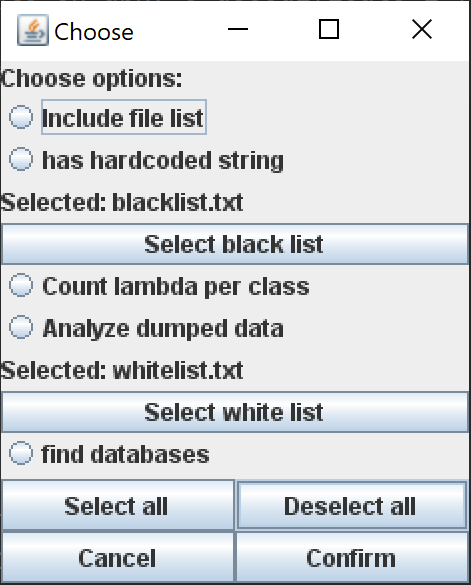
\includegraphics{./immagini/tool/analysis_chooser.png}
    \caption{Schermata delle opzioni dell'analisi}\label{fig:analysis_chooser}
\end{figure}
Di seguito è il codice che si occupa di "decorare" l'oggetto base, effettuare l'analisi e quindi generare un file pdf contenente il risultato:

\begin{lstlisting}[label={lst:analyze}]
public void analyze(Map< String, Boolean > thingsTodo, File blackList, File whiteList) {
        ...
Analyze analyze = new BaseAnalyzer(thingsTodo.get(AnalysisChooser.LIST_FILE), decompiledFiles);
...
// se analyzeString==true, allora analizzo le stringhe
if (thingsTodo.get(AnalysisChooser.FIND_STRING)) {
        analyze = new StringFinder(analyze, blackList);
}
        // se analyzeLambda==true, allora analizzo le lambda
if (thingsTodo.get(AnalysisChooser.COUNT_LAMBDA)) {
        analyze = new LambdaCounter(analyze);
}
        if (thingsTodo.get(AnalysisChooser.DUMPED_FILE)) {
        analyze = new DumpedFilesAnalyzer(analyze, whiteList);
}
        if (thingsTodo.get(AnalysisChooser.LIST_DBS)) {
        analyze = new DumpDataBase(analyze);
}
        ...
PDFWriter pdfWriter = new PDFWriter(resultFile);
pdfWriter.addParagraphs(analyze.getResult());
...
}
\end{lstlisting}

Con l'utilizzo del pattern decorator \`{e} estremamente semplice aggiungere un tipo di analisi, poiché è sufficiente aggiungere nella map \textit{thingsToDo} al momento della chiamata del metodo \textit{analyze}, creare una nuova classe che eredita dalla classe base dei decorator implementandone il metodo astratto e aggiungere due righe d'istruzione.

\subsection{Istanziazione di Commands}\label{subsec:istanziazione-di-commands}
Per il corretto funzionamento del tool è necessario che all'avvio venga instanziata una delle seguenti classi:
\begin{itemize}
    \item WindowsCommandFactory;
    \item LinuxCommandFactory.
\end{itemize}
Il seguente segmento di codice risolve tale problema:

\begin{lstlisting}[label={lst:commands}]
Commands commands;
String osInfo = System.getProperty("os.name");
if (containsIgnoreCase(osInfo, "windows")) {
    commands = new WindowsCommandFactory(model.getBasePath().getValue(), "cmd.exe", "/c");
} else {
    commands = new UnixCommandFactory(model.getBasePath().getValue(), "bash", "-c");
}
Controller controller = new Controller(model, commands);
\end{lstlisting}             % Product Prototype
    % !TEX encoding = UTF-8
% !TEX TS-program = pdflatex
% !TEX root = ../tesi.tex

%**************************************************************
\chapter{Verifica e validazione}
\label{ch:verifica-validazione}

\section{Analisi statica}\label{sec:analisi-statica}

L'analisi statica del codice\cite{site:analisi_static} è l'analisi del software che è effettuata senza eseguire
il codice.
Si pone in contrasto con l'analisi dinamica che invece richiede l'esecuzione del
programma.
Il termine è spesso utilizzato per indicare l'analisi eseguita da tool
automatici che nel caso del coinvolgimento dell'essere umano diventa code review.
Essa può  essere di due tipi, \gls{walkthrough} e \gls{inspection}.
Il tool utilizzato per l'analisi statica automatizzata è un plugin di Maven
chiamato checkstyle\cite{site:checkstyle} che è capace di generare un report indicando la presenza o
meno del codice che non è conforme alle convenzioni definite dal programmatore.

In questo progetto sono state definite le seguenti regole:
\begin{itemize}
    \item complessità delle espressioni booleane: al massimo 3;
    \item \gls{ciclomatica} delle funzioni: al massimo 16;
    \item lunghezza massima di ogni riga: 150 caratteri;
    \item lunghezza massima di ogni metodo: 100 righe;
    \item lunghezza massima di ogni file: 1000 righe;
    \item presenza dei blocchi di catch vuoi: vietata.
\end{itemize}

Il risultato dell'analisi è stato positivo, poiché non presenta nessuna riga del codice che non rispetti le regole sopracitate.

\section{Test unitari}\label{sec:test-unitari}
In ingegneria del software, per test d'unità si intende l'attività di testing delle singole parte unità del software.
Per unità si intende normalmente il componente più piccolo con funzionamento autonoma, quindi dipendentemente dal tipo di linguaggio di programmazione, l'unità può essere una funzione, una classe o un metodo.
Come le altre forme di test, i test d'unità può variare da completamente manuale ad automatico.
Specialmente nel caso dello unit testing automatico, lo sviluppo dei test case può essere considerato parte integrante dell'attività di sviluppo.\\

Nel caso del progetto \gls{apat} i test unitari sono stati fatti utilizzando il framework JUnit4\footcite{site:junit4} integrato con il tool di \gls{buildautomation} Maven\footcite{site:maven}.
\setcounter{rowcount}{0}

\newcounter{testCounter}
\setcounter{testCounter}{0}

\subsection{Specifica dei test}\label{subsec:specifica-dei-test-unitari}
Di seguito sono riportati i test d'unità che verificano il corretto funzionamento delle singole unità.
\begin{center}
    \begin{longtable}{ |C{3cm} | C{8.5cm}| C{1.5cm} |}
        \hline
        \textbf{Identificativo} &
        \textbf{Descrizione} &
        \textbf{Stato} \\\hline
        \idTest{TU} & Verificare che il file AndroidManifest.xml venga modificato correttamente.                              & I \\\hline
        \idTest{TU} & Verificare che dal file AndroidManifest.xml venga estratto il package corretto.                         & I \\\hline
        \idTest{TU} & Verificare che il nuovo path dell'APK venga aggiornato correttamente.                                   & I \\\hline
        \idTest{TU} & Verificare che la lista delle AVD venga ottenuta correttamente.                                         & I \\\hline
        \idTest{TU} & Verificare che l'AVD venga avviato con i parametri corretti.                                            & I \\\hline
        \idTest{TU} & Verificare che i file dex vengano decompilati correttamente.                                            & I \\\hline
        \idTest{TU} & Verificare che elenco dei file presenti nella cartella ./tmp sia corretto.                              & I \\\hline
        \idTest{TU} & Verificare che i file presenti nella cartella ./tmp vengano rimossi correttamente.                      & I \\\hline
        \idTest{TU} & Verificare che la ricompilazione dell'APK avvenga correttamente.                                        & I \\\hline
        \idTest{TU} & Verificare che la signing dell'APK ricompilato avvenga correttamente.                                   & I \\\hline
        \idTest{TU} & Verificare che l'apk venga installato correttamente nell'AVD.                                           & I \\\hline
        \idTest{TU} & Verificare che i dati scaricati dall'AVD siano quelli presenti nell'areas di storage dell'applicazione. & I \\\hline
        \idTest{TU} & Verificare che i file DEX vengano decompilati correttamente.                                            & I \\\hline
        \idTest{TU} & Verificare che il pdf generato sia corretto.                                                            & I \\\hline
        \idTest{TU} & Verificare che lo stato del tool caricato sia corretto.                                                 & I \\\hline
        \idTest{TU} & Verificare che lo stato del tool venga salvato correttamente.                                           & I \\\hline
        \idTest{TU} & Verificare che lo stato del tool venga resettato correttamente.                                         & I \\\hline
        \idTest{TU} & Verificare che i paragrafi venga inseriti nel pdf correttamente.                                        & I \\\hline
        \idTest{TU} & Verificare che il file zip venga estratto correttamente.                                                & I \\\hline
        \idTest{TU} & Verificare che il paragrafo generato corretto rispetto all'elenco dei file dati.                        & I \\\hline
        \idTest{TU} & Verificare che il paragrafo generato corretto rispetto all'elenco dei file dati.                        & I \\\hline
        \idTest{TU} & Verificare che il paragrafo generato corretto rispetto all'elenco dei file dati.                        & I \\\hline
        \idTest{TU} & Verificare che il paragrafo generato corretto rispetto all'elenco dei file dati.                        & I \\\hline
        \idTest{TU} & Verificare che il commando generato per decompilare l'APK sia corretto.                                 & I \\\hline
        \idTest{TU} & Verificare che il commando generato per ricompilare l'APK sia corretto.                                 & I \\\hline
        \idTest{TU} & Verificare che il commando generato per firmare l'APK ricompilato sia corretto.                         & I \\\hline
        \idTest{TU} & Verificare che il commando generato per ottenere l'elenco delle AVD sia corretto.                       & I \\\hline
        \idTest{TU} & Verificare che il commando generato per avviare l'AVD sia corretto.                                     & I \\\hline
        \idTest{TU} & Verificare che il commando generato per installare l'APK sull'AVD sia corretto.                         & I \\\hline
        \idTest{TU} & Verificare che il commando generato per scaricare l'area di storage dell'app installato sia corretto.   & I \\\hline
        \idTest{TU} & Verificare che il commando generato per convertire i file .class in .java sia corretto.                 & I \\\hline
        \idTest{TU} & Verificare che il commando generato per rimuovere i file decompilati sia corretto.                      & I \\\hline
        \idTest{TU} & Verificare che il commando generato per connettersi all'AVD come root sia corretto.                     & I \\\hline
        \idTest{TU} & Verificare che il commando generato per connettersi all'AVD normalmente sia corretto.                   & I \\\hline
        \idTest{TU} & Verificare che il commando generato per ottenere i parametri del terminale sia corretto.                & I \\\hline
        \idTest{TU} & Verificare che la mappa restituita contenga esattamente le scelte dell'utente.                          & I \\\hline
        \idTest{TU} & Verificare che vengano accettati solo i file di tipo APK.                                               & I \\\hline
        \idTest{TU} & Verificare che la descrizione restituita sia corretta.                                                  & I \\\hline
        \idTest{TU} & Verificare che vengano accettati solo i file di tipo KJS.                                               & I \\\hline
        \idTest{TU} & Verificare che la descrizione restituita sia corretta.                                                  & I \\\hline
        \idTest{TU} & Verificare che vengano accettati solo i file di tipo TXT.                                               & I \\\hline
        \idTest{TU} & Verificare che la descrizione restituita sia corretta.                                                  & I \\\hline
        \idTest{TU} & Verificare che la stringa restituita sia corretta.                                                      & I \\\hline
        \idTest{TU} & Verificare che l'elenco dei file ottenuto sia corretto.                                                 & I \\\hline
        \idTest{TU} & Verificare che l'arrotondamento avviene correttamente.                                                  & I \\\hline
        \caption{Test d'unità}
    \end{longtable}
\end{center}
\setcounter{rowcount}{0}

\subsection{Tracciamento}\label{subsec:tracciamento-unitari}
\begin{center}
    \begin{longtable}{ |C{3cm} |C{10.5cm}|}
        \hline
        \textbf{Identificativo} &
        \textbf{Componente} \\\hline
        \idTest{TU} & AndroidManifest.editDebugAttribute()       \\\hline
        \idTest{TU} & AndroidManifest.getPackageName()           \\\hline
        \idTest{TU} & Controller.updateApkPath()                 \\\hline
        \idTest{TU} & Controller.refreshAVDList()                \\\hline
        \idTest{TU} & Controller.startAvd()                      \\\hline
        \idTest{TU} & Controller.decompile()                     \\\hline
        \idTest{TU} & Controller.listFolderElements()            \\\hline
        \idTest{TU} & Controller.removeDecompiledFiles()         \\\hline
        \idTest{TU} & Controller.recompile()                     \\\hline
        \idTest{TU} & Controller.signAPK()                       \\\hline
        \idTest{TU} & Controller.installCompiledApk()            \\\hline
        \idTest{TU} & Controller.dumpDataFromAVD()               \\\hline
        \idTest{TU} & Controller.decodeDex()                     \\\hline
        \idTest{TU} & Controller.analyze()                       \\\hline
        \idTest{TU} & Controller.loadState()                     \\\hline
        \idTest{TU} & Controller.saveState()                     \\\hline
        \idTest{TU} & Controller.resetModelState()               \\\hline
        \idTest{TU} & PDFWriter.addParagraphs()                  \\\hline
        \idTest{TU} & Unzipper.unzip()                           \\\hline
        \idTest{TU} & DumpDataBase.doAnalysis()                  \\\hline
        \idTest{TU} & DumpedFilesAnalyzer.doAnalysis()           \\\hline
        \idTest{TU} & LambdaCounter.doAnalysis()                 \\\hline
        \idTest{TU} & StringFinder.doAnalysis()                  \\\hline
        \idTest{TU} & Commands.getDecompileCommand()             \\\hline
        \idTest{TU} & Commands.getCompileApkCommand()            \\\hline
        \idTest{TU} & Commands.getSigningApkCommand()            \\\hline
        \idTest{TU} & Commands.getListOfAvds()                   \\\hline
        \idTest{TU} & Commands.getStartAvdCommand()              \\\hline
        \idTest{TU} & Commands.getInstallAPK()                   \\\hline
        \idTest{TU} & Commands.getDumpApplicationDataCommand()   \\\hline
        \idTest{TU} & Commands.getConvertToJavaCommand()         \\\hline
        \idTest{TU} & Commands.getRemoveDecompiledFilesCommand() \\\hline
        \idTest{TU} & Commands.connectToAdbAsRoot()              \\\hline
        \idTest{TU} & Commands.getAttachToAvdCommand()           \\\hline
        \idTest{TU} & Commands.getCli()                          \\\hline
        \idTest{TU} & Analysis.chooser()                         \\\hline
        \idTest{TU} & APKFilter.accept()                         \\\hline
        \idTest{TU} & APKFilter.getDescription()                 \\\hline
        \idTest{TU} & KeystoreFilter.accept()                    \\\hline
        \idTest{TU} & KeystoreFilter.getDescription()            \\\hline
        \idTest{TU} & TxtFilter.accept()                         \\\hline
        \idTest{TU} & TxtFilter.getDescription()                 \\\hline
        \idTest{TU} & Utils.getDate()                            \\\hline
        \idTest{TU} & Utils.listAllFiles()                       \\\hline
        \idTest{TU} & Utils.round()                              \\\hline
        \caption{Tracciamento dei test d'unità}
    \end{longtable}
\end{center}

I test sopraelencati sono stati superati con successo, con una \gls{codecoverage} del \textit{84.2\%}.


             % Product Design Freeze e SOP
    % !TEX encoding = UTF-8
% !TEX TS-program = pdflatex
% !TEX root = ../tesi.tex

%**************************************************************
\chapter{Conclusioni}
\label{ch:conclusioni}
%**************************************************************
\intro{}

% !TEX encoding = UTF-8
% !TEX TS-program = pdflatex
% !TEX root = ../tesi.tex

%**************************************************************
\section{Consuntivo finale}\label{sec:consuntivo-finale}

% !TEX encoding = UTF-8
% !TEX TS-program = pdflatex
% !TEX root = ../tesi.tex

%**************************************************************
\section{Raggiungimento degli obiettivi}\label{sec:raggiungimento-degli-obiettivi}

% !TEX encoding = UTF-8
% !TEX TS-program = pdflatex
% !TEX root = ../tesi.tex

%**************************************************************
\section{Conoscenze acquisite}\label{sec:conoscenze-acquisite}

% !TEX encoding = UTF-8
% !TEX TS-program = pdflatex
% !TEX root = ../tesi.tex

%**************************************************************
\section{Valutazione personale}\label{sec:valutazione-personale}             % Conclusioni
    \appendix
    % !TEX encoding = UTF-8
% !TEX TS-program = pdflatex
% !TEX root = ../tesi.tex

%**************************************************************
\chapter{Appendice A}
%**************************************************************

\epigraph{Citazione}{Autore della citazione}



             % Appendice A

%**************************************************************
% Materiale finale
%**************************************************************
    \backmatter
    \printglossaries
    % !TEX encoding = UTF-8
% !TEX TS-program = pdflatex
% !TEX root = ../tesi.tex

%**************************************************************
% Bibliografia
%**************************************************************

\cleardoublepage
\chapter{Bibliografia}\label{ch:bibliografia}

\nocite{*}
% Stampa i riferimenti bibliografici
\printbibliography[heading=subbibliography,title={Riferimenti bibliografici},type=book]

% Stampa i siti web consultati
\printbibliography[heading=subbibliography,title={Siti web consultati},type=online]


\end{document}
